
\chapter{量子计算简介}
很久很久以前,在一个不知名的国度,一个男人被判了死刑。他要求觐见国王,国王也同意听这个男人最后说几句话。“如果你让我再活一年,”男人说道,“我保证我会让您的马飞起来。”
国王非常好奇,也非常期待能拥有一匹这个国家唯一的能飞的马,于是他就给了这个男人一年的生命。

当男人回到家把这个事情告诉他的妻子的时候,她大喊道:“你疯了!你不可能让马飞起来的!”男人很从容地解释道:“你说的是对的,马是不会飞的。但你要知道一年的时间什么都有可能发生。国王可能会死,国家可能会卷入战争,国王的马也可能会死,但我至少可以再多活一年。”

在本章中,我们会先介绍经典计算机遭遇的瓶颈,然后会回顾量子计算发展的历史,并简要阐述量子计算机的工作模式。最后,我们会介绍量子计算机的各种可能的物理实现的进展,这正是开始故事的寓意所在。
\label{chap:introduction}
    \section{经典计算机将到达极限}
    “\emph{当价格不变时,在一块集成电路上可容纳的晶体管数目,大概每隔18个月会翻一倍,而其性能也会翻倍。}”

 \hspace{23em} \emph{--戈登·摩尔}


让我们把时钟拨回到四年前。

2008年2月19日,苹果公司产品发布会。当时依然精神矍铄的苹果总裁史蒂夫·乔布斯兴正在致勃勃的和全世界谈他今天要讲的
第四件事情。他神秘的拿出了一个牛皮信封,告诉大家产品就在这个信封里。所有现场的观众都感到好奇,可能全世界的观众也在好奇,
魔术师一般的乔帮主这次到底要拿出什么震惊世界的产品。大家凝神屏息之时,乔布斯从牛皮信封里缓缓抽出了一张炫目的银色画图板。
恐怕谁都不会想到,这居然是一台性能优秀的笔记本电脑,而它又是如此之轻薄,最薄之处仅有4mm,最厚也不过19.4mm,拿在手里就像一片银色的树叶一样。

关于苹果家族的新成员Macbook Air的这段传奇搬的历史在此已无需赘述,苹果早已以其无限的创意和惊人的实力震撼了全世界。如今,乔老爷子已经仙逝,众多知名的电脑公司
也已经可以惟妙惟肖地模仿Air的造型。但人们还是不禁要问,我们的电脑在不损失性能的前提下,到底还能瘦身到什么程度?1965年,时任Intel名誉总裁的摩尔早就
有了一个非凡的论断:在单个集成电路芯片上能够放置的晶体管数目,大约在一年半内翻一番。迄今为止,这个定律还没有饱和,但是如果利用摩尔定律往下推论,
大概到2020年,我们必须要用原子尺寸来储存单个比特的信息。学过量子力学的人都知道,量子效应在那时候将占支配性的地位。

经典计算机遇到的第二个不可回避的问题是,它在本质上是耗散的。换句话说,经典计算机所有的计算过程都是不可逆的,每擦除一个比特的信息,都要在损耗能量
上付出一定的代价。很多人都有过把笔记本电脑当做小型电暖气来使用的经历,也曽碰到因为散热问题过于严重导致电脑罢工的情况。当芯片的尺寸做的更小时,这个损耗会更加明显。
Landauer在1961年就已提出\cite{Landauer},如果要擦除一个比特的信息,耗散的周围环境的热能至少是$k_BTln2$。其中,$k_B$ 是Boltzman常数,$T$是经典计算机周围环境的温度。事实上,当前的计算机每执行一个经典逻辑门的能量要比这个值高一个数量级以上。
        \begin{figure}[htbp]
            \begin{center}
              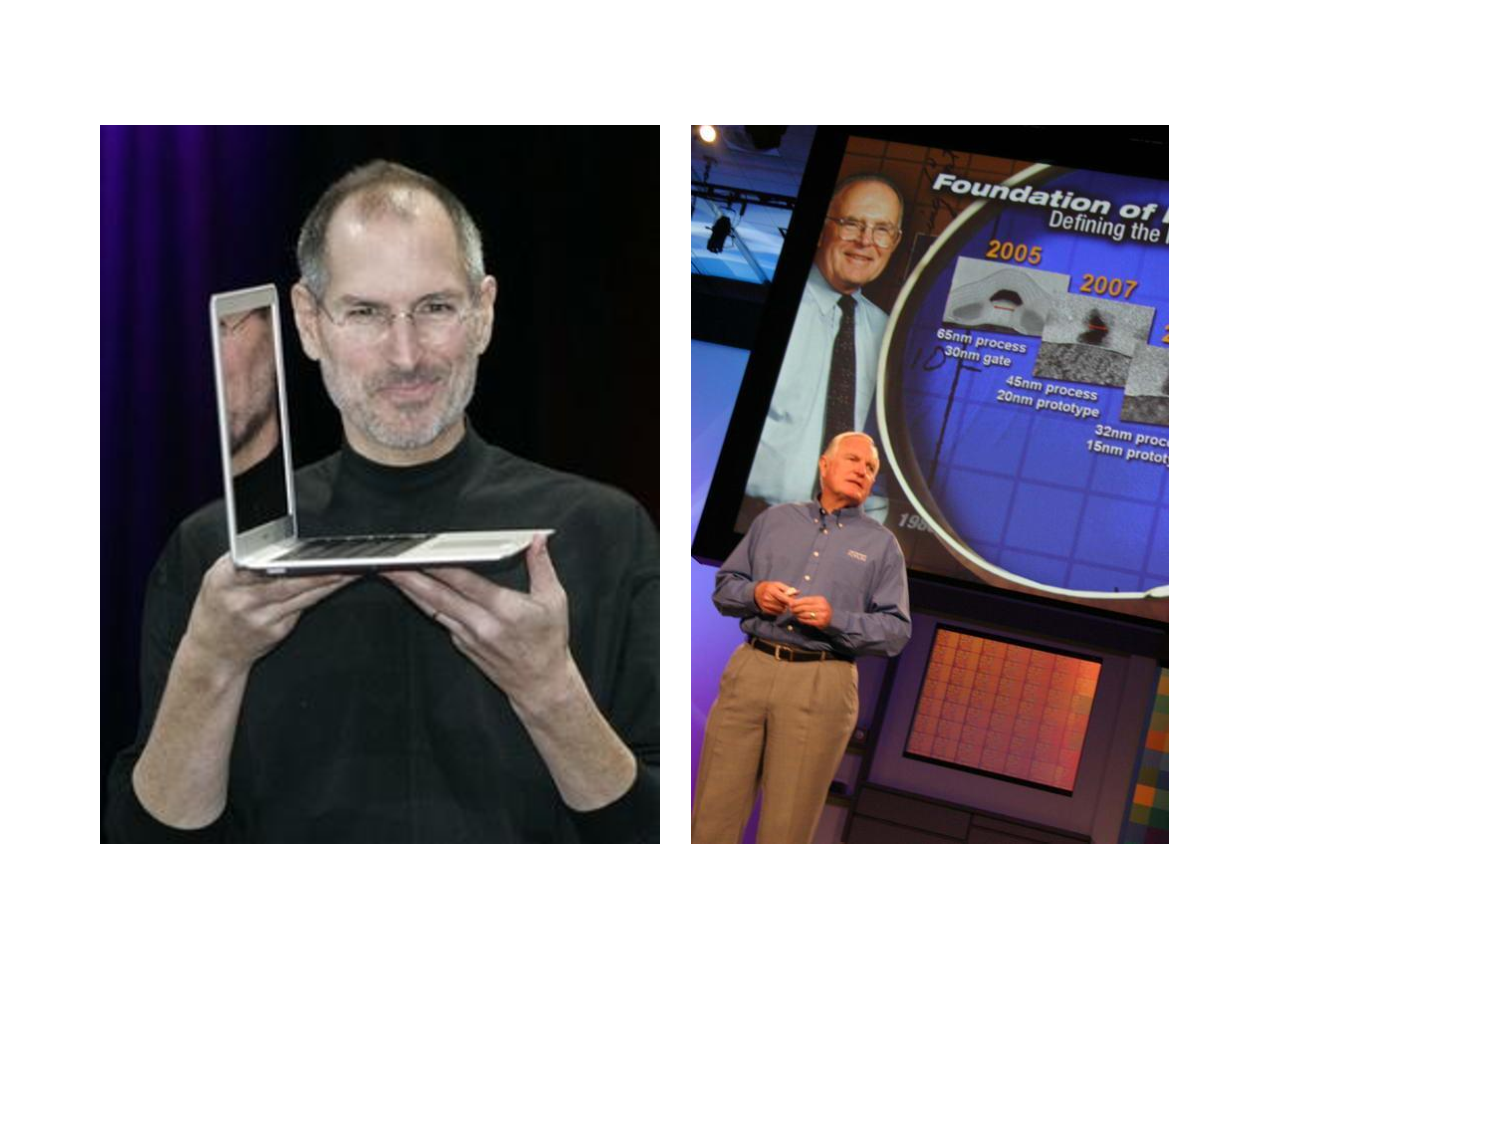
\includegraphics[width= 0.8\columnwidth]{figures/jobs.pdf}
              \caption{(左)乔布斯以及薄如蝉翼的Macbook Air;(右)摩尔定律的提出者戈登·摩尔在演讲
              }
              \label{jobs}
            \end{center}
        \end{figure}

    量子效应和热耗散是经典计算机继续发展下去不可回避的问题。其实,还有一个问题是:经典计算机的
    计算能力极限是多少?一个简单的例子就能说明问题。3乘5等于15,这是一个六七岁的孩子都能回答上的问题。但反过来,15等于
    几乘几呢?虽然这依然是个简单的问题,但它却蕴含了一个可怕的事实:原则上来说经典计算机对这个问题是无能为力的!用科学点的话
    来讲,如果要用经典计算机处理质因数分解的问题,它所需求的时间是指数增长的,在数学上这种问题属于不可求解问题。我们不妨利用一下
    所谓的质因数分解问题来考验一下经典计算机。

    20世纪50年代,真空管计算机大概能够进行每秒1000次的浮点运算,而到了2005年,超级计算机已经可以每秒执行百万亿次的浮点运算,这是一个非常惊人的数字。
    那么,如果我们要分解一个512位的整数需要多久呢?这看上去对我们信赖的计算机应该不是什么难事,但答案却是令人诧异的。如果我们选择每秒能够处理百万次运算的
    芯片,那么这个时间将是8400年!即使使用最强劲的超级计算机,时间花费依然要一个小时之久。如果我们要分解的整数位数增加,计算机分解它所耗费的时间
    更是指数增加的。所以,质因数分解算法是当前最主流的加密算法RSA公钥所采用的加密形式,理论上来说它是牢不可破的,也广泛被应用于政府、军队、银行等重要部门。



    \section{量子计算的应运而生}

    “\emph{底下的空间还大得很。}”

 \hspace{23em} \emph{--理查德·费曼}

其实用应运而生这个词并不准确。量子计算的概念并不是因为经典计算即将到达瓶颈而提出来的。当1959年量子计算的概念第一次提出时\cite{Feynman},经典计算机也只能算刚刚起步(第一台经典计算机Eniac问世于1946年)。
在这次著名的演讲中,费曼给物理学家和工程师们提出了一个有趣的挑战:在\emph{\textbf{很小}}的尺度上
进行操作和控制。特别地,他让听众思考我们能不能建立一种计算机,它的导线直径只有约10到100个原子,而电路仅仅有几百纳米这么大?五十年过去了,现在的半导体工艺已经很接近这个尺度,但费曼的本义并不仅仅是指小,
而是非常非常的小,小到人们要开始考虑量子力学法则:

\emph{“当我们涉及非常,非常小的世界时,比如说7个原子的电路,就会有些有趣的事情出现,可能给予我们新的设计思路。小尺度上的原子行为和大尺度上一点都不同,因为它们仅仅满足量子力学法则。
所以,当我们涉足这个世界的时候,我们必须改变我们的看法,因为我们在和不同的法则一起工作,而这很可能导致我们可以做很多不同的事情。当然,不仅是电路,我们也可以采用一些其他的系统,比如分离的能级,自旋间的相互作用等等。”}

这应该是最早具有量子计算雏形的思想,它充分结合了当时最热门的学科-量子力学的各种推论,描绘了一幅非常诱人的图景。而费曼更是同时给了一个著名的论断:

\emph{“我并不是想违背什么法则。这只是原则上我们可以做到的事情,我们现在还没做到是因为我们实在太大了。”}

经典计算机碰到的下一个问题就是热耗散。既然Landauer认为热耗散来自于逻辑门的不可逆性,那只要说明量子计算是可逆的就可以完全避免这个问题了。Lecerf \cite{Lecerf} 和 Bennett \cite{Bennett}证明,确实可以找到普适的可逆计算,不需要擦除信息,从而也不会产生热耗散。后来, Benioff \cite{Benioff} 发现量子力学的哈密顿量可以被用作普适的经典图灵机模型。换句话说,基于量子力学哈密顿量演化的量子计算是无热耗散的。

真正提出量子计算优越性的还是费曼 \cite{Feynman2,Feynman3}。他认为量子计算机依靠有效模拟其他量子系统的演化,可以做到很多经典图灵机做不到的事情。接着Deutsch发展完善了所谓的量子图灵机模型,并指出量子计算机具有
通过量子并行性来加速计算的潜力 \cite{Deutsch}。

十年之后,量子计算领域第一个真正通过量子并行性取得指数加速的算法,也是让全世界感到震惊的算法-Shor算法 \cite{Shor} 横空出世。之所以说让全世界感到震惊,是因为如上一小节所说,
大多数的部门机构都是采用RSA密钥系统加密,而RSA密钥系统的依据就是大数不能在经典上被有效分解。相对于每秒百万次运算的经典计算机需要8400年来分解一个512位的整数,Shor算法仅需3.5个小时就能
做到这一点!正是由于量子计算的特殊叠加和相干性质,Shor算法可以在多项式的时间复杂度内解决大数分解问题,这在算法上被称作是有效的。该算法提出后,每个国家都会担心自己的安危,一旦在这场信息战中输掉,可能整个国家最
重要的机密就泄露了。也正是由于Shor算法,很多国家都大大增加了量子计算实验研究的投入,因为它的回报实在太大了。

在开始量子计算的全面介绍之前,我们先通过一个耳熟能详的例子展望下量子计算机将怎样改变人们的生活。在文明出现以前,人类就学会了使用光。从最早的摩擦生火产生的火光,到后来的蜡烛和灯笼,再到电发明后
产生的灯泡,所有这些光都有一个共同的性质:非相干性(incoherence)。20世纪60年代,第一台激光器问世了。可能当时谁都不会想到这个在中国被音译为“镭射”的东西会在接下来的半个世纪内给人类带着这么多变化,甚至于夸张点说,
改变了这个世界。最快的刀,最准的尺,最亮的光,无穷无尽的应用,无穷无尽的奇思妙想。你可以用它来逗一下自己的小猫,也可以看球时带着它干扰一下对方的球员;你可以在枪上安装个瞄准镜做到“十步杀一人,千里不留名”,也可以
模仿一下阿纳金,玩一把《星球大战》的cosplay秀。这些都是科学外的应用,而这一切的应用都源于激光的一个性质-相干性(coherence)。

        \begin{figure}[htbp]
            \begin{center}
              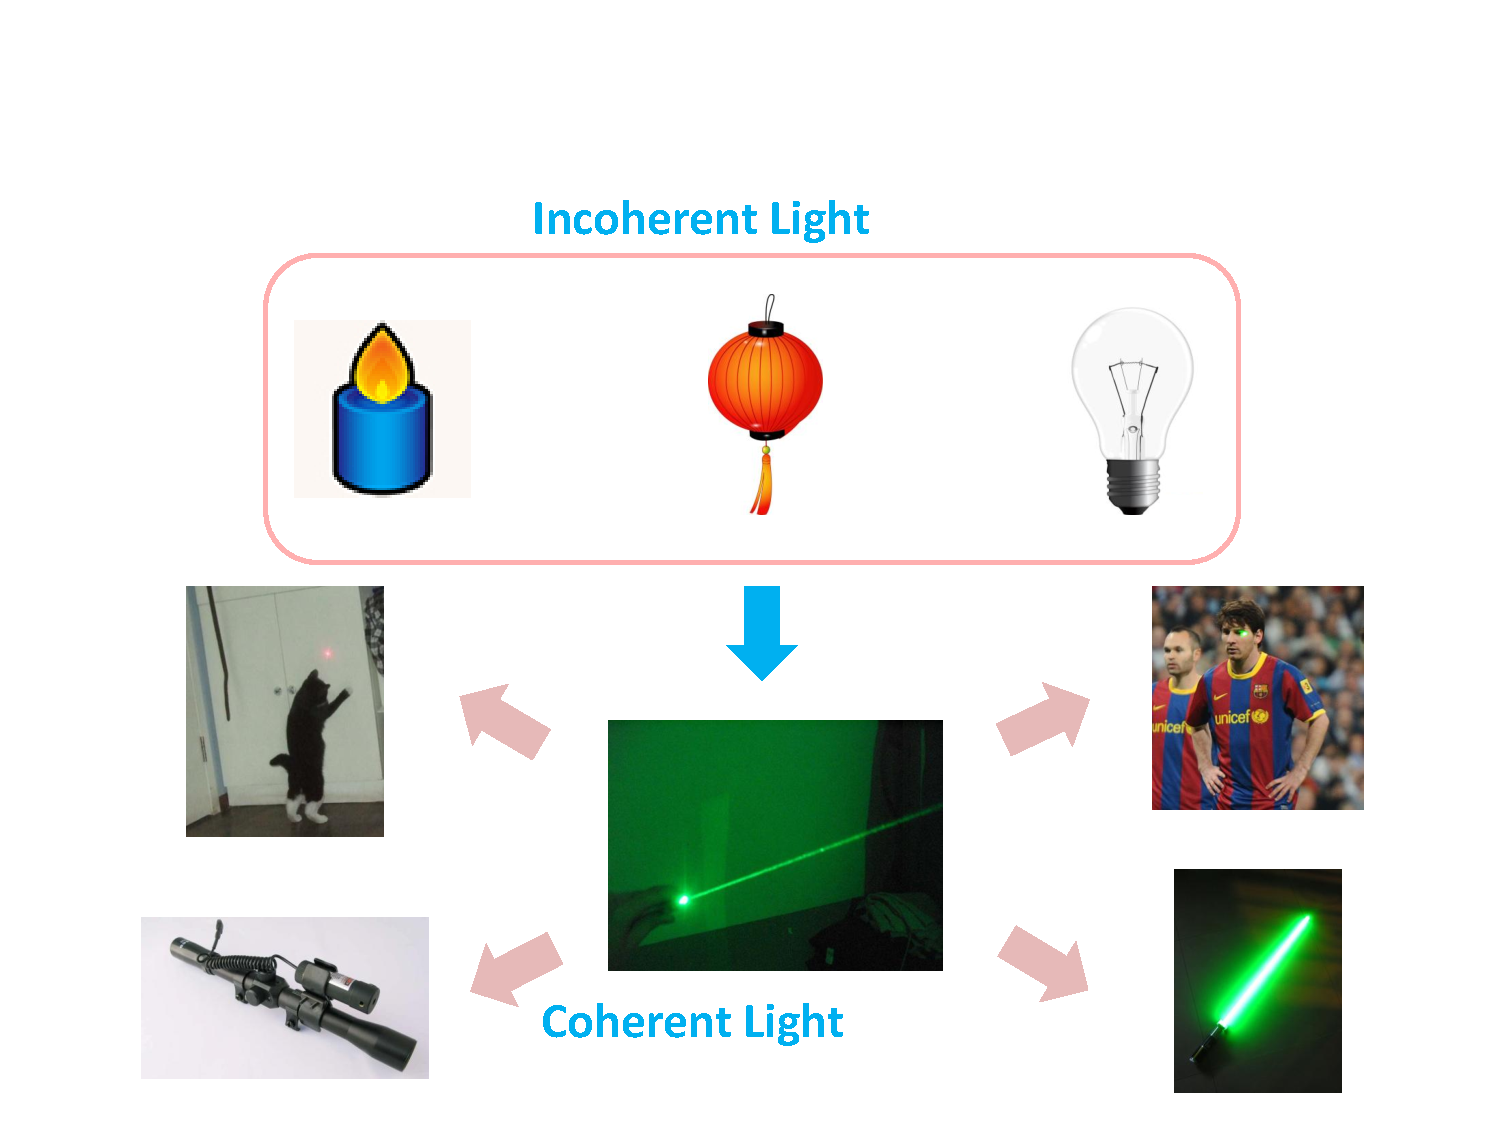
\includegraphics[width= 0.8\columnwidth]{figures/laser.pdf}
              \caption{从非相干光到相干光,人类的生活发生了巨大的改变。从非相干的经典图灵机到相干的量子计算机,人类又将迎来怎样的变化呢?
              }
              \label{laser}
            \end{center}
        \end{figure}

        就如同激光并不是一种新型的经典光,量子计算机也不是新型的经典计算机。它并不能说是快的,或者小的进化型经典计算机,它的进化决不是从电脑到笔记本电脑再到平板电脑的进化这么简单,它将会是一种具有
        全新模式的计算机。指导它工作的不再是长串的01编码,而是量子力学演化。我们想象不到有了量子计算机后生活将发生怎样翻天覆地的变化,目前我们最主要的任务只是
        让这个变化尽早发生。

    \section{量子计算机的工作原理}

    “\emph{当你改变你观看世界的方法的时候,你看到的世界也在改变。}”

 \hspace{23em} \emph{--马克·普朗克}

    在本节中,我们将讨论量子计算的线路模型。事实上,也有更抽象的图灵机模型,两者在物理上是等价的。

    \subsection{量子比特}

    在经典图灵机模型中,储存经典信息的基本单位叫做比特。它是一个二进制变量,其数值一般记做二进制的0或者1。一个比特要么是0,要么是1,正如向空中抛起一枚硬币,那么它落下后
    要么正面朝上,要么反面朝上。我们用二进制的比特理论上可以储存任何信息,最简单的,储存十进制整数就可以利用二进制和十进制的转换。 3=11, 4=100, 50 =110010等等。当然,非整数也是可以写成二进制的形式,像5.5 = 101.1,也就是说任意实数都可以按精度要求用二进制来表示。而在电子学中,很多器件是非常适合二进制表示的,例如电压的高低和开关,电容器的带电荷与否等等,都可以来作为一个比特的载体。

但在量子世界,一切都发生了改变。一个量子的硬币不仅可以正面或反面朝上,它甚至可以同时正反面都朝上,在你观测它之前。著名的薛定谔的猫就是这个道理,这只猫在开箱子,也就是观测之前,它又是死的又是
活的,处于生和死的\emph{\textbf{叠加态}} (superposition state) 上。正是叠加性这个奇妙的性质引出了量子比特(quantum bit, qubit) 的概念。一个量子比特可以认为是一个在二维希尔伯特空间 (Hilbert space) 中描述的两能级量子体系,它可以在数学上被表示为
\begin{equation}
           \left\vert \psi \right\rangle= \alpha  \left\vert 0 \right\rangle + \beta  \left\vert 1 \right\rangle.
 \end{equation}
其中,振幅$\alpha$和$\beta$是任意复数,且满足归一化条件
\begin{equation}
          |\alpha|^2 + |\beta|^2 =1.
 \end{equation}
$\left\vert \psi \right\rangle$就是一个$\left\vert 0 \right\rangle$ 和$\left\vert 1 \right\rangle$的叠加态。$\left\vert \psi \right\rangle$的定义中含有一个不能被任何测量手段观测到且没有物理意义的整体相位,因此我们可以把$\left\vert \psi \right\rangle$写成
 \begin{equation}
           \left\vert \psi \right\rangle= cos\frac{\theta}{2}  \left\vert 0 \right\rangle + e^{i\phi}sin\frac{\theta}{2}  \left\vert 1 \right\rangle.
 \end{equation}
在几何上,我们可以把这个态表示为一个球面上的点,这个球就叫做Bloch球,见Fig. \ref{bloch}。这种基于量子力学的表示形式很容易让人联想到拥有两个自由度$\theta$和$\phi$的经典模拟变量(analog variable),但一个量子比特和经典模拟变量有本质的不同:一个处于 $\left\vert 0 \right\rangle$和 $\left\vert 1 \right\rangle$的叠加态上
的量子比特,从某种意义上来说,是同时处在$\left\vert 0 \right\rangle$态和$\left\vert 1 \right\rangle$态上的!薛定谔猫的概念就是用一种很通俗的说法描述了
量子比特这种奇妙的叠加性。更进一步讲,在一个$n$-qubit的态上,它的自由度是和$n$成指数增长关系的。很快我们就会看到这一点。

        \begin{figure}[htbp]
            \begin{center}
              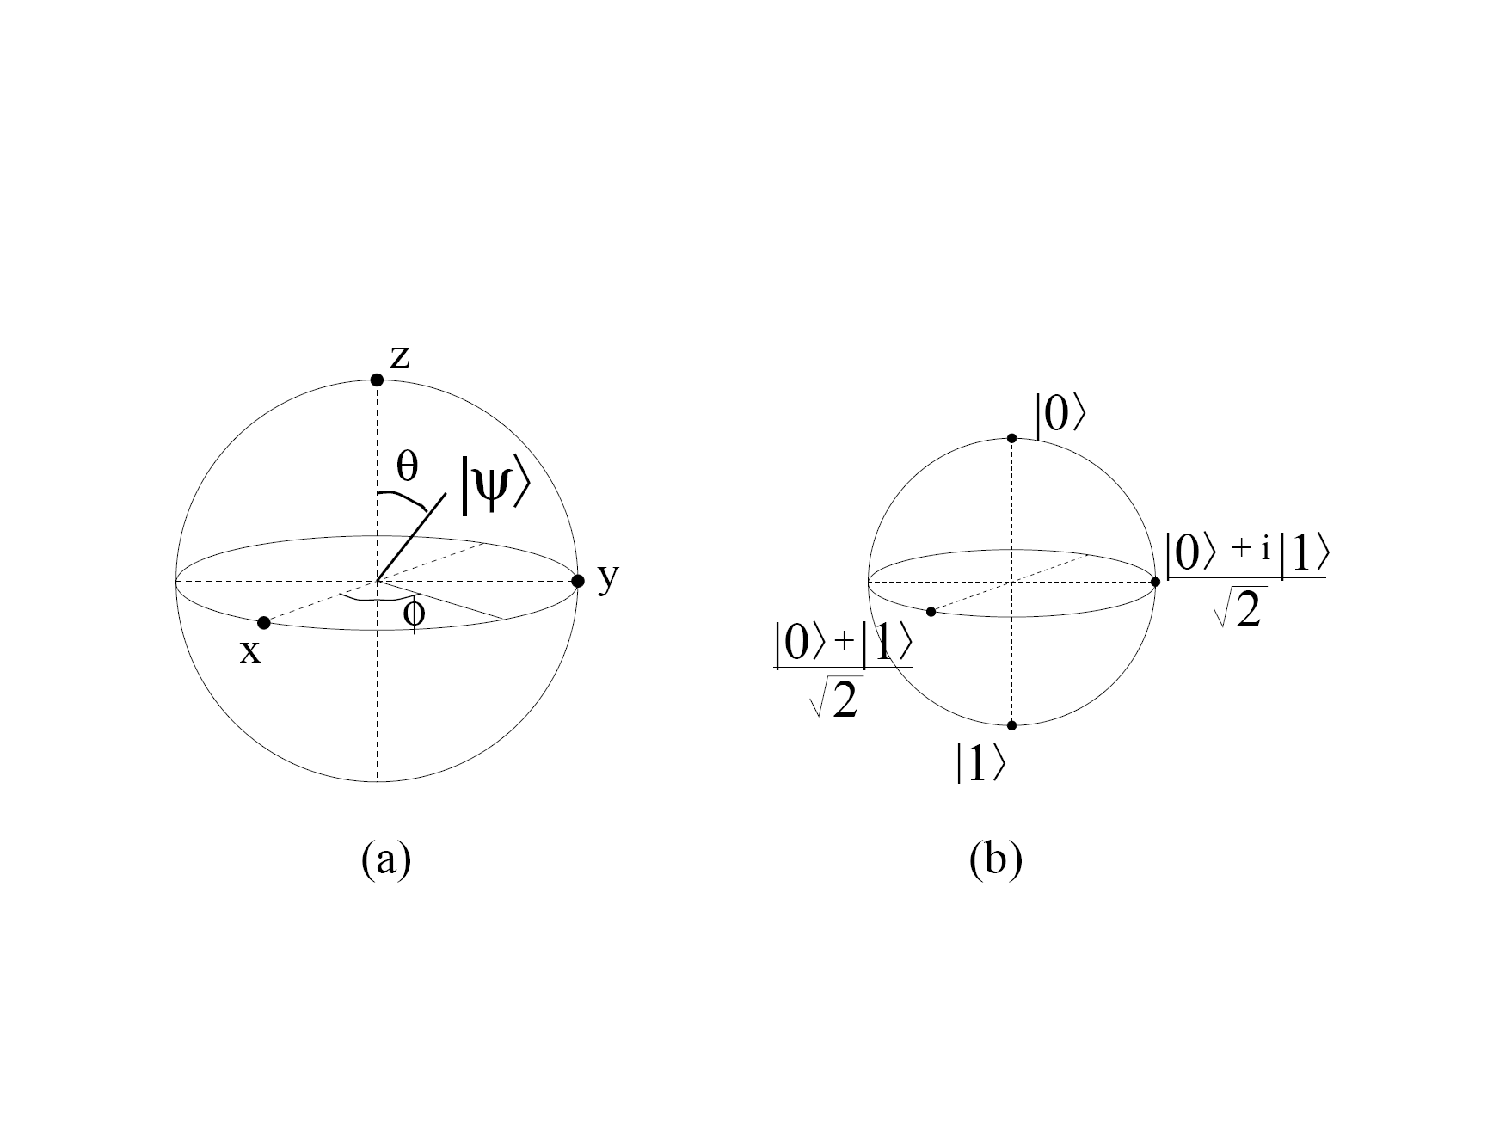
\includegraphics[width= 0.8\columnwidth]{figures/bloch.pdf}
              \caption{(a) 单比特态$ \left\vert \psi \right\rangle$可以用Bloch球上的一个点来表示。(b) Bloch球上的4个重要的点。一般我们把 $\left\vert 0 \right\rangle$态定义为$+\hat{z}$方向。
              }
              \label{bloch}
            \end{center}
        \end{figure}

两个比特的态,假设每一个都处于任意叠加态$ \left\vert \psi \right\rangle_1= \alpha_1  \left\vert 0 \right\rangle + \beta_1  \left\vert 1 \right\rangle$ ,$ \left\vert \psi \right\rangle_2= \alpha_2  \left\vert 0 \right\rangle + \beta_2 \left\vert 1 \right\rangle$ ,则这两个比特的状态可以写成
 \begin{equation}
           \left\vert \psi \right\rangle=\left\vert \psi_1 \right\rangle \otimes \left\vert \psi_2 \right\rangle= (\alpha_1  \left\vert 0 \right\rangle + \beta_1  \left\vert 1 \right\rangle)\otimes( \alpha_2  \left\vert 0 \right\rangle + \beta_2 \left\vert 1 \right\rangle),\label{sepa}
 \end{equation}
 其中$\otimes$是张量积符号,或者叫做直积符号(Kronecker product)。把上式展开,我们能够得到
   \begin{equation}
           \left\vert \psi \right\rangle=  \alpha_1  \alpha_2 \left\vert 0 \right\rangle \otimes \left\vert 0 \right\rangle+\alpha_1  \beta_2 \left\vert 0 \right\rangle \otimes \left\vert 1 \right\rangle+\beta_1  \alpha_2 \left\vert 1 \right\rangle \otimes \left\vert 0 \right\rangle+\beta_1  \beta_2 \left\vert 1 \right\rangle \otimes \left\vert 0 \right\rangle.
 \end{equation}
为了方便,后面我们将省略直积符号$\otimes$, 并把$\left\vert 0 \right\rangle \otimes \left\vert 0 \right\rangle$ 简记为$\left\vert 00 \right\rangle$,以此类推。因此,
 \begin{equation}
           \left\vert \psi \right\rangle=  \alpha_1  \alpha_2 \left\vert 00 \right\rangle +\alpha_1  \beta_2 \left\vert 01 \right\rangle +\beta_1  \alpha_2 \left\vert 10 \right\rangle+\beta_1  \beta_2 \left\vert 11 \right\rangle.
 \end{equation}
 那么,对一个$n$-qubit的寄存器,它的状态可以写成$2^n$个态的叠加,
  \begin{equation}
           \left\vert \psi \right\rangle=  \sum _{i=0}^{2^n-1}c_i \left\vert k \right\rangle.
 \end{equation}
  对这个态的唯一约束条件是归一化条件:
   \begin{equation}
             \sum _{i=0}^{2^n-1} |c_i|^2 =1.
 \end{equation}
 和单比特情形类似,整体相位是可以忽略的。因此,要描述一个$n$-qubit 的纯态需要$2^n-1$个复变量 (混态情形是$4^n-1$个自由度,此处不作详细讨论)。

 在物理实现上,原则上具有叠加性质的两态量子系统都适用做qubit。目前的实验室里,像NMR中
 处于磁场中的自旋1/2粒子(自旋向上和向下),空腔中的原子的态(原子的基态和激发态),超导结之间隧穿的库珀对(Cooper pairs处于一个结和另外一个结时),都可以被用作qubit。当然,如果一个硬币可以同时向上和向下也是可以的,在量子随机行走
 中我们就会看到这种量子硬币(quantum coin)。

 现在我们可以回过头来在看一下经典计算机和量子计算机的差距,这次是存储容量上的。
 考虑一个简单的情况,我们要储存45个自旋1/2的粒子,这在量子系统中只是一个很小的体系,只需要45个qubit就可以实现。但如果我们要用经典
 计算机完成这个任务,约需要$2^{45}$个经典比特,也就是大概4个TB的硬盘!这里有些典型的数据来跟它比较,4TB大概是4,000G或者4,000,000M,而一部高清蓝光电影大概是10G,一本书大概是5M,编写本论文的Tex软件包
也只有2G。另外一些比较有意思的数据是,美国国会图书馆的所有藏书总容量大概为160TB或者说50个qubit,而2007年人类所拥有的信息量总和为$2.2\times 10^9$个TB
\cite{Hilbert},也仅相当于71个qubit的存储容量。
 \begin{figure}[htbp]
            \begin{center}
              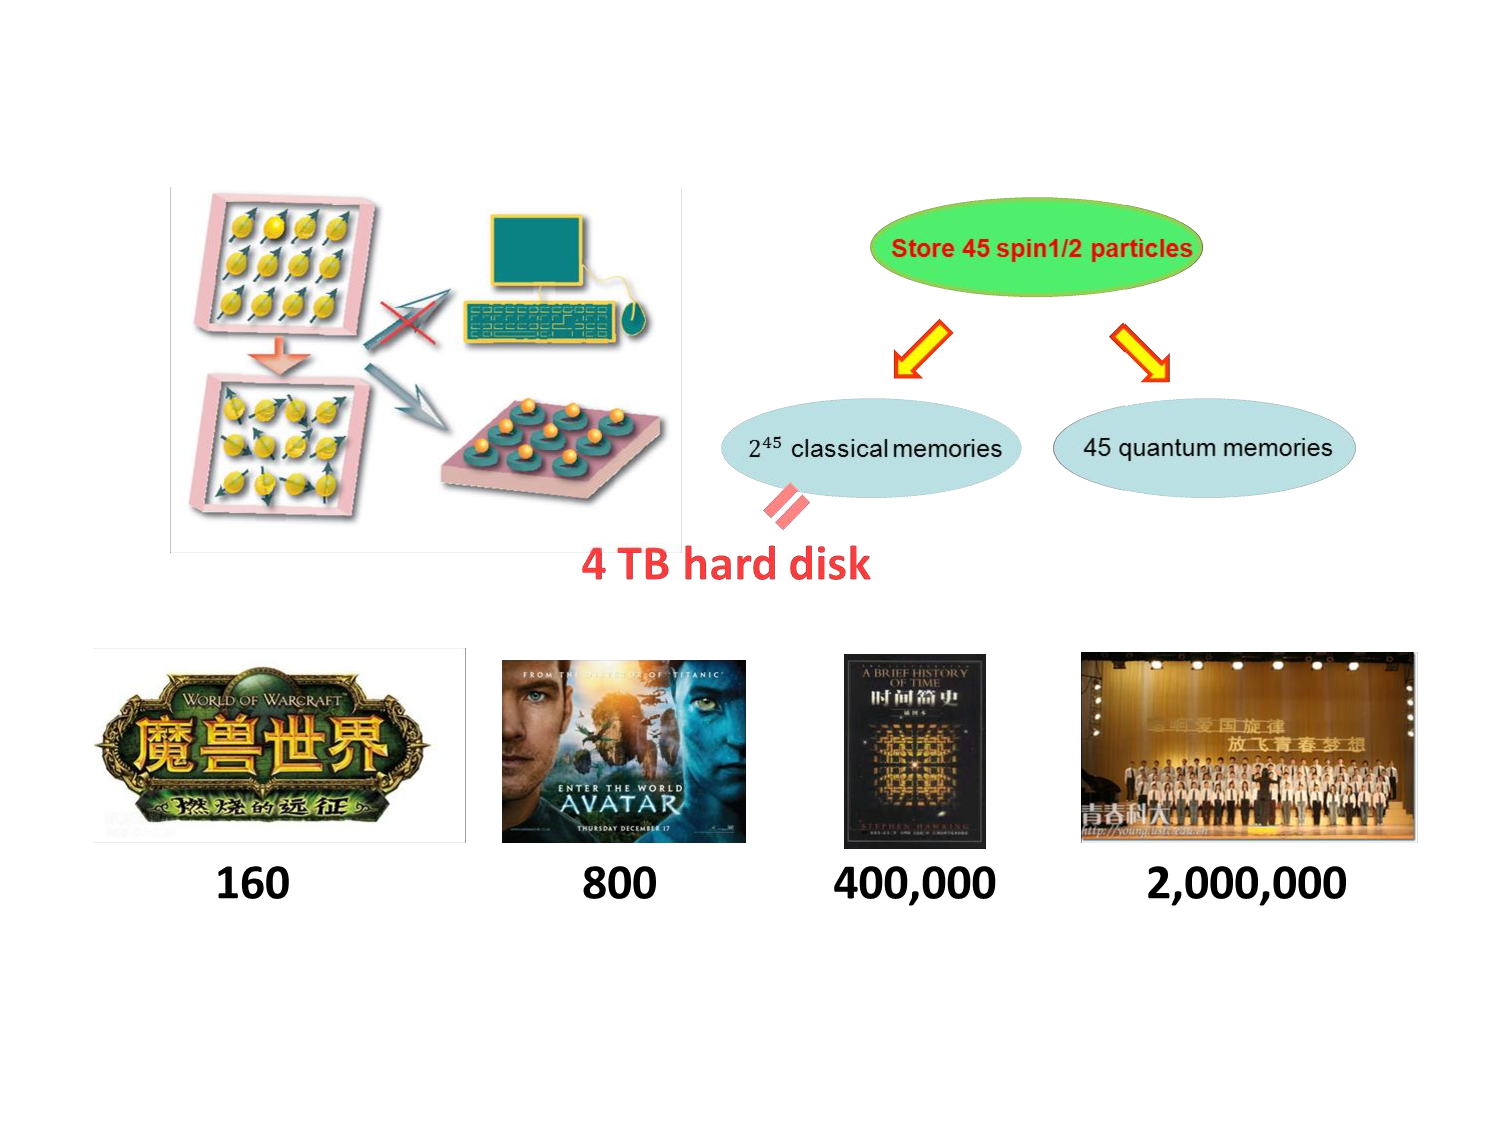
\includegraphics[width= 0.8\columnwidth]{figures/register.pdf}
              \caption{要储存45个自旋1/2的粒子,我们需要45个量子比特或者$2^{45}$个
              经典比特。用这些经典比特组成的硬盘我们可以做很多事情,比如存放160个《魔兽世界》,800部
              《阿凡达》,40万本《时间简史》或者200万首《永恒的东风》。仅仅从存储量上看,经典计算机已经输了。
              }
              \label{register}
            \end{center}
  \end{figure}

\subsection{量子纠缠}

虽然叠加原理赋予了量子计算机 可以在一次运行中完成指数次运算的机会, 也就是并行性计算模式,但叠加性并不是量子系统独有的。事实上,也存在满足叠加性原理的经典波,比如两端固定的弦震动方程。但和量子系统不同的是,这些所谓的叠加
能级必须属于同一个系统,属于不同系统的经典态是永远不能叠加起来的,也就是没有\textbf{纠缠}(entanglement)的。如果一个多比特量子态能够被
写成各个比特的态的直积形式,那么我们就说这个态是可分离(separable)的,比如Eq. \ref{sepa} 。

相反地,我们总可以找到合适的$\alpha_1, \beta_1$和$\alpha_2, \beta_2$,使得$ \left\vert \psi \right\rangle_1= \alpha_1  \left\vert 0 \right\rangle + \beta_1  \left\vert 1 \right\rangle$ 和$ \left\vert \psi \right\rangle_2= \alpha_2  \left\vert 0 \right\rangle + \beta_2 \left\vert 1 \right\rangle$ 直积之后的结果为
 \begin{equation}
         \frac{\left\vert 00 \right\rangle+ \left\vert 11 \right\rangle}{\sqrt{2}},
 \end{equation}
 那么不论我们如何分解,它都是不可能被写成两个qubit的态的直积形式的。这种情况我们就称这个态是不可分离(non-separable)的或者\textbf{纠缠}(entangled)的。后面我们会看到,
 纠缠是量子计算中最重要的资源之一,绝大部分的量子算法加速都源于量子纠缠。当然,近些年有理论研究表明纠缠并不是量子算法加速必不可少的资源,还存在着一种
 叫做量子无序(quantum discord)的资源比纠缠的实用范围更加广泛,具体这部分研究可以参考其他文献。

 \subsection{量子态的演化和量子逻辑门}

 前面我们给出了量子比特的\textbf{静态}性质,讲了量子寄存器的存储方法以及重要的量子纠缠资源。这一小节我们将着重于研究怎么用一种可控的方式来实现我们的
 计算任务,也就是量子比特的\textbf{动态}性质。

 在一个封闭的量子系统中,态的演化是满足薛定谔方程的
  \begin{equation}
         i\hbar \frac{d\left\vert \psi(t)\right\rangle}{dt}=H\left\vert \psi(t)\right\rangle,
 \end{equation}
其中 $\hbar$是普朗克常数,$H$是整个系统的哈密顿量。对于不含时(time-independent)的哈密顿量来说,
薛定谔方程有很简单的解
   \begin{equation}
       \left\vert \psi(t)\right\rangle = e^{-iHt/\hbar} \left\vert \psi_0\right\rangle,
 \end{equation}
 $\psi_0$是$t=0$时系统所处的态。一般,我们用幺正算子$U$来定义时间演化算子,即
    \begin{equation}
       U = e^{-iHt/\hbar},
 \end{equation}
 也就是说,
   \begin{equation}
       \left\vert \psi(t)\right\rangle =U \left\vert \psi_0\right\rangle.
 \end{equation}
 如果用密度矩阵的语言,那么量子系统的密度矩阵演化可以写成
    \begin{equation}
       \rho(t) = \left\vert \psi(t)\right\rangle \left\langle \psi(t)\right\vert = U\rho_0 U^{\dagger}.
 \end{equation}
 在后面的章节中,为了方便我们将把普朗克常数$\hbar$的值设为1。

 一般来说,在简单的量子系统中,一般包含单粒子项和两粒子间的相互作用项。三体及以上的相互作用
 至今还没在实验中被观测到。因此,我们能够实现的量子逻辑门都是单比特门或两比特门。很幸运的是,
 后面我们将看到,任何幺正操作$U$都是可以拆解成单量子门和\textbf{受控}两比特门的组合的 \cite{Deutsch2,DiVincenzo2,Lloyd2,DBE}。 我们将在下面分别讨论单量子们和两比特门。

 最简单的单比特门是非门(NOT gate)。和经典情况类似,非门的作用是可以把 $\left\vert 0\right\rangle$ 和 $\left\vert 1\right\rangle$ 相互翻转。非门的矩阵形式是
     \begin{equation}
       U_{NOT} = \left(
                   \begin{array}{cc}
                     0 & 1 \\
                     1 & 0 \\
                   \end{array}
                 \right).
 \end{equation}
 如果输入态是任意态
  \begin{equation}
       \left\vert \psi\right\rangle =\left(
                                                                       \begin{array}{c}
                                                                         \alpha \\
                                                                         \beta \\
                                                                       \end{array}
                                                                     \right),
 \end{equation}
 那么非门作用后
      \begin{equation}
       U_{NOT}\left\vert \psi\right\rangle = \left(
                   \begin{array}{cc}
                     0 & 1 \\
                     1 & 0 \\
                   \end{array}
                 \right)\left(
                                                                       \begin{array}{c}
                                                                         \alpha \\
                                                                         \beta \\
                                                                       \end{array}
                                                                     \right) = \left(
                                                                       \begin{array}{c}
                                                                         \beta \\
                                                                         \alpha \\
                                                                       \end{array}
                                                                     \right).
 \end{equation}
 另外一种重要的单比特量子门叫做Hadamard门,其定义为
      \begin{equation}
       H =\frac{1}{\sqrt{2}} \left(
                   \begin{array}{cc}
                     1 & 1 \\
                     1 & -1 \\
                   \end{array}
                 \right).
 \end{equation}
 经过Hadamard门后,$\left\vert 0\right\rangle$ 和 $\left\vert 1\right\rangle$将分别变成 $\left\vert +\right\rangle$ 和 $\left\vert -\right\rangle$ ,即
   \begin{eqnarray}
       &&H\left\vert 0\right\rangle =\frac{1}{\sqrt{2}} (\left\vert 0\right\rangle+\left\vert 1\right\rangle)\equiv \left\vert +\right\rangle,\nonumber \\
        &&H\left\vert 1\right\rangle =\frac{1}{\sqrt{2}} (\left\vert 0\right\rangle-\left\vert 1\right\rangle)\equiv \left\vert -\right\rangle.
 \end{eqnarray}

 实际上。任意的单比特操作都可以写成如下形式
 \begin{equation}
      U = e^{i\alpha}R_{\hat{n}}(\theta),
 \end{equation}
 其中$R_{\hat{n}}(\theta)$对应于Bloch球上的旋转操作,绕$\hat{n}=(n_x,n_y,n_z)$轴旋转$\theta$角。
 在定义了泡利矩阵(Pauli matrices)后
 \begin{equation}
      \sigma_x\equiv \left(
                       \begin{array}{cc}
                         0 & 1 \\
                         1 & 0 \\
                       \end{array}
                     \right),  \sigma_y\equiv \left(
                       \begin{array}{cc}
                         0 & -i \\
                         i & 0 \\
                       \end{array}
                     \right),  \sigma_z\equiv \left(
                       \begin{array}{cc}
                         1 & 0 \\
                         0 & -1 \\
                       \end{array}
                     \right),
\end{equation}
我们就可以把单比特旋转操作用泡利算子展开
\begin{equation}
    R_{\hat{n}}(\theta)\equiv e^{-i\frac{\theta\hat{n}\cdot\overrightarrow{\sigma}}{2}}  = cos(\theta/2)\sigma_I - isin(\theta/2)[n_x \sigma_x+n_y \sigma_y+n_z \sigma_z].
\end{equation}

两比特门中最常见的是控制非门(controlled-NOT gate, CNOT gate)。在CNOT门中第一个比特起控制作用,第二个比特为目标比特。当控制比特处于 $\left\vert 0\right\rangle$时,受控非门不进行操作。当控制比特处于 $\left\vert 1\right\rangle$时,目标比特进行翻转操作。CNOT门的作用可以表示成
 \begin{equation}
    U_{CNOT} \left\vert \psi_1\right\rangle \left\vert \psi_2\right\rangle = \left\vert \psi_1\right\rangle \left\vert \psi_1\oplus \psi_2\right\rangle (\psi_1,\psi_2 = 0,1),
\end{equation}
$\oplus$是模2操作。写成矩阵形式的话,CNOT门是$4\times4$的
 \begin{equation}
    U_{CNOT} = \left(
                 \begin{array}{cccc}
                   1 & 0 & 0 & 0 \\
                   0 & 1 & 0 & 0 \\
                   0 & 0 & 0 & 1 \\
                   0 & 0 & 1 & 0 \\
                 \end{array}
               \right).
\end{equation}
该形式为比特1控制比特2的CNOT门形式。还有一种重要的两比特门叫做SWAP门,它的作用
是把两个比特的状态进行交换,值得注意的是SWAP门不是受控的。它的矩阵形式是
 \begin{equation}
    U_{SWAP} = \left(
                 \begin{array}{cccc}
                   1 & 0 & 0 & 0 \\
                   0 & 0 & 1 & 0 \\
                   0 & 1 & 0 & 0 \\
                   0 & 0 & 0 & 1 \\
                 \end{array}
               \right).
\end{equation}

主要的两比特门在量子线路图中用如下符号表示:
\begin{figure}[htbp]
            \begin{center}
              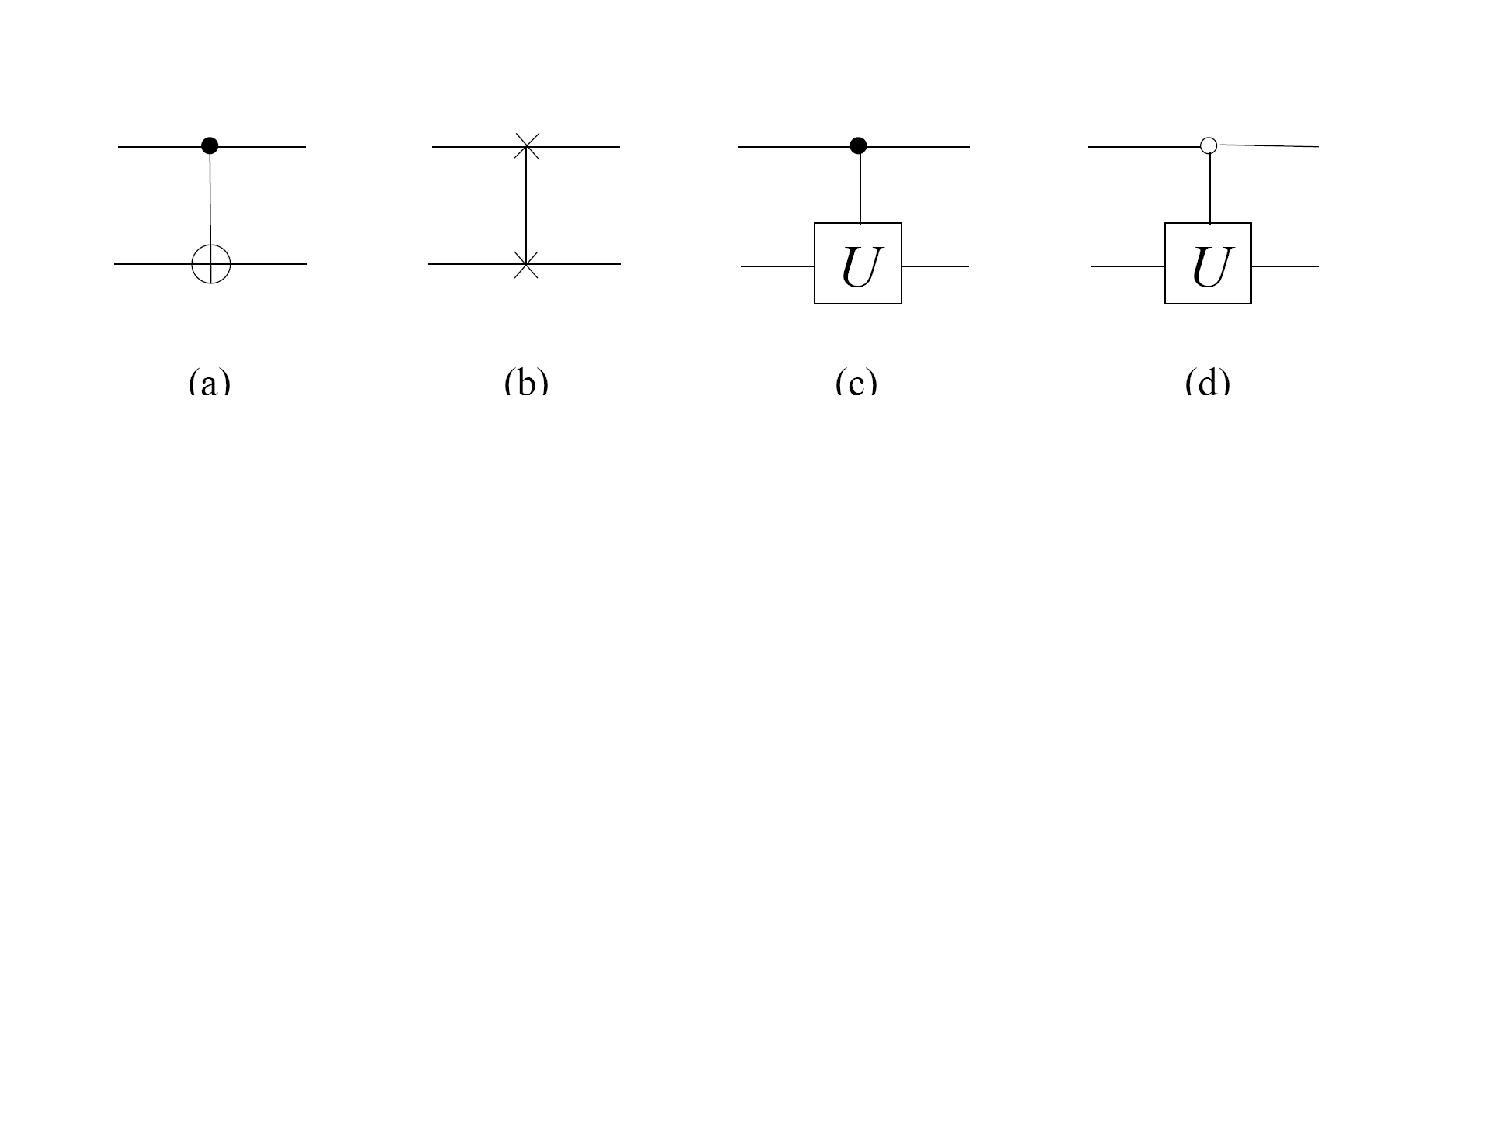
\includegraphics[width= 0.8\columnwidth]{figures/cnot.pdf}
              \caption{几种常用的两比特量子门(a) CNOT$_{12}$门,(b) SWAP门,(c) 控制U门,(d) 0控制U门。
              }
              \label{cnot}
            \end{center}
  \end{figure}

事实上,对于多比特系统,更重要的是如下关于量子线路分解的定理:

\emph{任意的量子门都可以分解为CNOT门和单比特旋转门的组合。}

有了以上定理,如果我们能找到有效的分解算法,那么原则上我们可以实现
任意复杂的量子线路图。

\subsection{量子态的测量}

在量子力学的假设中,对一个量子系统的任意测量操作总可以用一组测量算子
$P_m$来描述。对一个处于$\left\vert \psi\right\rangle$态的量子系统,经过观测算子 $P_m$后得到结果为$m$的概率为
\begin{equation}
    p(m) =\left\langle \psi \right\vert P_m \left\vert \psi\right\rangle.
\end{equation}
测量后,该量子系统将塌缩为
\begin{equation}
    \frac{P_m \left\vert \psi\right\rangle}{\left\langle \psi \right\vert P_m \left\vert \psi\right\rangle}.
\end{equation}
这组测量算子的集合必须满足完备性关系
\begin{equation}
  \Sigma_m P_m = I,
\end{equation}
才能保证所有概率$p(m)$之和为1。特别的,对于投影测量(projective measurement),我们还要求 $P_m$是厄米算子并且
\begin{equation}
P_m P_{m'} = \delta_{mm'}P_m.
\end{equation}
因此,我们可以利用一组正交基$\left\vert m \right\rangle$来定义任意投影算子的集合,简单的比如$P_m = \left\vert m \right\rangle \left\langle m \right\vert $。在这组投影测量下,得到$m$的概率为
 \begin{equation}
    p(m) = |\left\langle m \right\vert \psi  \rangle |^2,
\end{equation}
且测量后的态为$\left\vert m \right\rangle$。

如果我们在$\{ \left\vert 0 \right\rangle , \left\vert 1 \right\rangle\}$基中测量单比特态$ \alpha  \left\vert 0 \right\rangle + \beta  \left\vert 1 \right\rangle$ ,那么我们得到$\left\vert 0 \right\rangle$ 的概率为$|\alpha|^2$,得到$\left\vert 1 \right\rangle$ 的概率为$|\beta|^2$。

当然Stern-Gerlach实验早就证明对于量子系统被测量后的塌缩性质,也就是我们
不可能通过对一个qubit进行连续测量来得到其系数$\alpha$和$\beta$。当然,一个直接的
想法是如果我们可以在大量该粒子的拷贝上进行足够多的投影测量,总能通过统计规律
得到$\alpha$和$\beta$的值。但很遗憾,不可克隆定理(no-cloning theorem)\cite{Dieks,nocloning}告诉我们这也是不行的,因为我们不能对一个处于未知态的
qubit进行精确的拷贝(或许可以预见盗版量子计算机的软件将是一个技术活)。 总结来说,

\emph{没有测量手段可以完全揭示一个处于未知态的量子比特的状态。}

关于量子计算的基本原理的参考书目及文献很多。值得推荐的有:

Nielsen和Chuang的名作《量子计算与量子信息》\cite{yellow},国内被昵称为“黄书”(因其中文版封面为黄色);
非常基础的Steane写的review \cite{steane},当然这篇文献的部分内容已经非常过时;
Preskill的讲稿 \cite{Preskill};Bennett和DiVincenzo写的权威性评述 \cite{benben};Benenti, Casati和Strini合著的《量子计算与量子信息原理》\cite{wangwenge}(中文版为王文阁,李保文等译)。

\section{量子计算机的物理实现}

    “\emph{我们要记住,或许有一天量子理论会被证明是失败的,因为它和我们日常的生活经验、哲学是如此的不同。}”

 \hspace{23em} \emph{--理查德·费曼}

上一节的内容已经从理论上大致描绘了一台量子计算机的蓝图,但在真正的量子计算机问世之前,一切都是空话。
理论上已经提出了很多方案可以物理实现量子计算,但对大规模量子系统的精确控制存在着很多困难,比如退相干效应。在宏观
世界中,我们很难观测到量子行为的一个重要原因就是退相干已经把量子性彻底给退光了。但是,随着技术的日新月异以及更有潜力的量子计算方案的提出,
人们距离真正的量子计算机还是越来越近的。2011年,加拿大的D-Wave公司就宣称他们已经成功研制了世界上第一台通用量子计算机 \cite{dwave},包含128个qubit,售价为1000
万美金。美国的Lockheed Martin公司斥巨资购买了一台,但业内人士对这个号称基于绝热量子计算的庞然大物 普遍存在质疑,认为它并不能做到真正的单qubit控制,且能解决的任务非常有限。本文不会对这个争议颇多的“量子计算机”作更多的讨论,更重要的是分析当前各量子计算方案的利弊,
力图给出各方案的发展前景。

 \begin{figure}[htbp]
            \begin{center}
              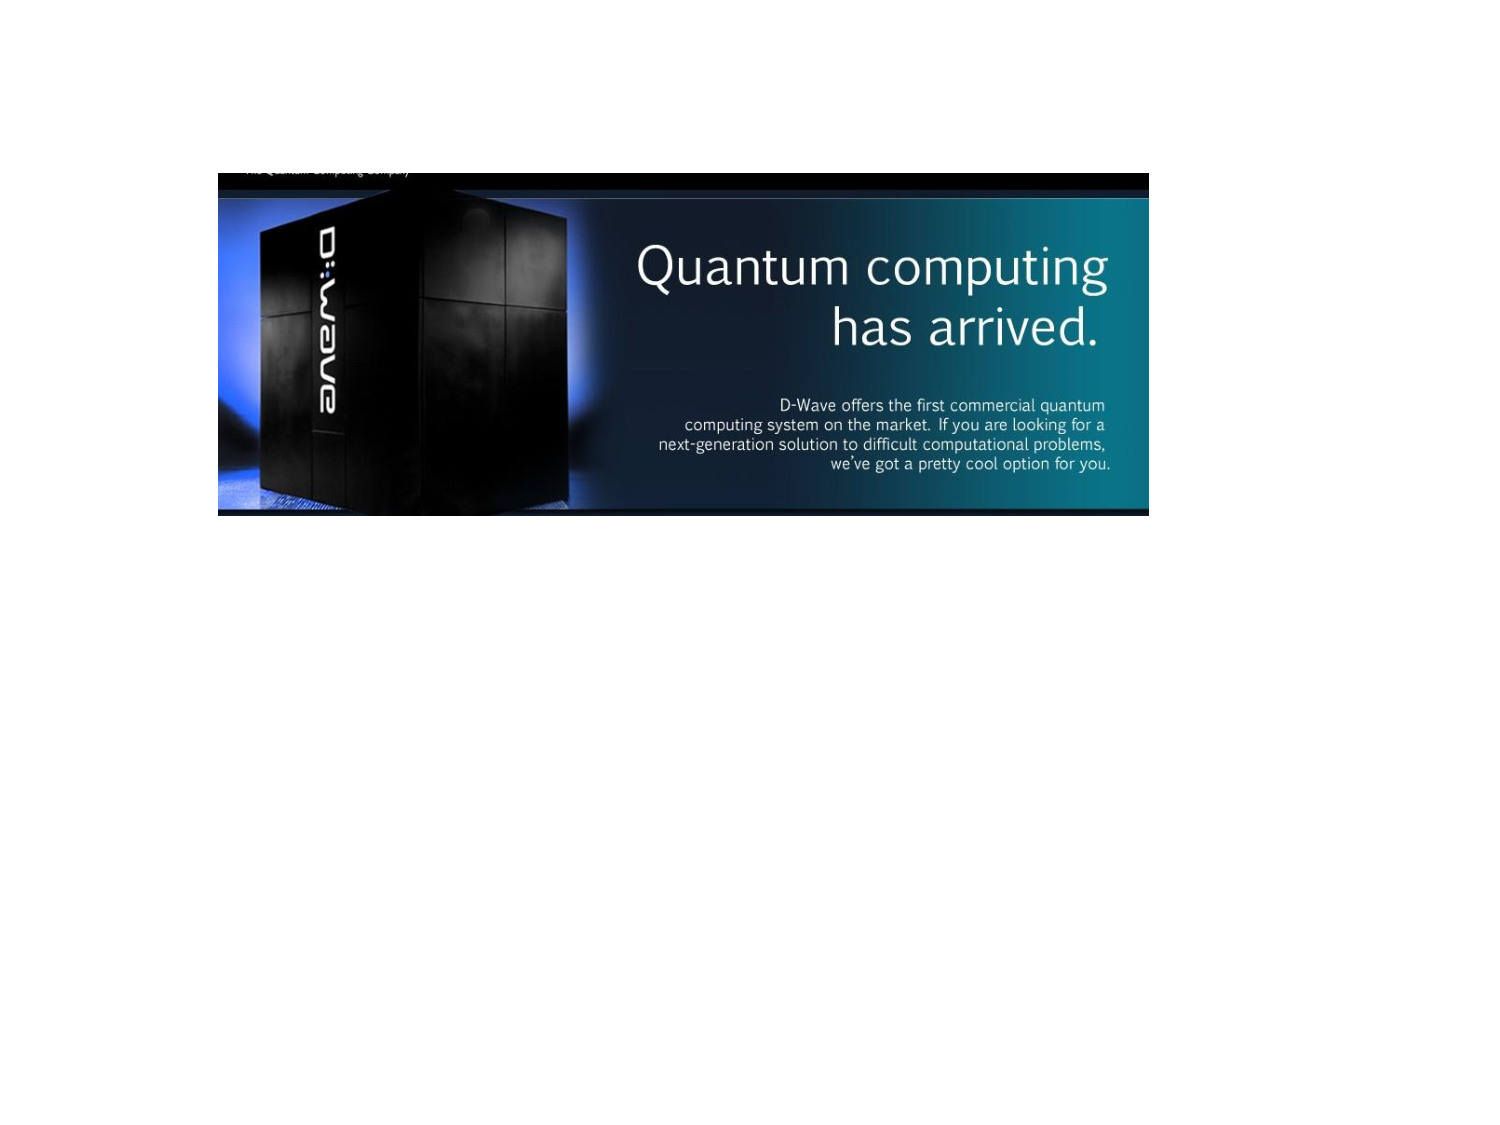
\includegraphics[width= 0.8\columnwidth]{figures/dwaveqc.pdf}
              \caption{加拿大D-Wave公司宣称他们已经制造出第一台128-qubit的超导量子计算机,但谁也不知道这个售价高的吓人(1000万美金)的超大黑盒子里藏的是什么。
              }
              \label{dwave}
            \end{center}
  \end{figure}

  \subsection{量子计算机的要求}

或许对量子计算机最苛刻,也是最普适的要求是所谓的“封闭盒子”(close box)条款:在操作人员的控制下所执行的量子计算机的内部操作,必须和整个宇宙的其他部分孤立开来。即使一点点的干扰都可能让我们脆弱的量子计算机产生毁灭性的
衰亡,也就是\textbf{退相干}(decoherence)。

退相干有多种来源。在大量实验的系综测量中,由于哈密顿量是含时的,导致每次的振荡频率总会有差别,统计下来整个设备就会有信号衰减,这个时间尺度叫做$T_2^{\ast}$;实验中,系统总会被附加一些随机的过程或者放出能量,
导致统计结果为系统朝热平衡态演化,这个时间尺度叫做$T_1$;而系统也可能和外界环境通过相互作用让振荡产生相位扰动,导致相干的衰减,这个时间尺度叫做$T_2$。一般来说,$T_2\leq 2T_1$,而且在绝大多数系统中,$T_1 \gg T_2$,所以在量子计算中$T_2$是更加重要的。

没有什么系统是完全的退相干不变的,但是少量的退相干影响是可以通过各种技术消除的,著名的比如\textbf{量子纠错}(quantum error correction)。早期的对容错量子计算机的物理实现要求有著名的DiVencenzo五条定则\cite{DiVincenzo5},这里不再赘述。如果我们假设物理体系的退相干效应足够小的话, 一个物理实现方案只需要满足下面三个条件就可以用做量子计算机的潜在体系了。

首先是\textbf{可扩展性}(scalablity)。量子计算机的操作都是在Hilbert空间中进行的,而Hilbert的空间维度是指数形式增长的,这就要求我们的物理体系要有非指数的资源,但却
能反应出Hilbert空间的指数增长,例如时间,空间,能量等。标准的做法就是遵循 DiVincenzo的第一条定则:可以简单的对一个系统增加新的且可分辨的qubit。当然要宣称一个方案是“可扩展的”确实非常难,因为用来定义和操控qubit的资源总是多种多样的,这会涉及到很多经典技术,比如
微芯,微波,激光,低温等。为了证明该方案可扩展,必须同时要把这些技术做到可扩展,这可能就需要非常复杂的工科知识了。

其次是该体系有能执行\textbf{普适的逻辑操作}。也就是,在大的Hilbert空间中的操作必须能够分解成一系列简单的操作,而这些简单操作的需求资源不能是指数增长的。当然,前面已经
说过,任意角度的单比特旋转门和两比特CNOT门就可以组合成任意的逻辑操作,也就是说只要该体系能够有效实现这两个门就可以了。当然,出了基于逻辑门的量子计算,还有其他的量子计算模式,比如
绝热量子计算(adiabatic quantum computation)\cite{adia1},单向量子计算(one-way quantum computation)\cite{oneway1}等。这些量子计算模式中和基于逻辑门的量子计算是等价的,但执行它们并不需要拆解逻辑门。

最后是\textbf{纠错能力}(correctability)。该方案必须能够萃取计算机的信息熵来得到有用的量子态,比如有效的初态制备和测量。初态制备其实就是把一个量子系统迅速
地冷却到低熵的状态,而测量就是迅速地以较高的精度得到量子系统的状态的能力,这两者在某种意义上是相似的,且已经被统一到了量子纠错理论中。

目前建造量子计算机最主要的挑战就是操控,测量量子系统的能力,以及阻止系统和外界环境的相互作用的能力,我们将对目前主流的备选方案进行基本介绍。

  \subsection{光学量子计算}

相比于其他系统,光子的退相干效应要小很多,非常适合用作qubit。qubit的信息可以编码到光子的极化状态上,而单比特旋转可以通过线性光学器件,如分束器,相移器等 轻松实现,但如何达到需求的相互作用
从而实现两比特门一直是一个难题,采用非线性Kerr介质中的原子来传递在技术上非常困难。2001年,著名的KLM(Knill-Laflamme-Milburn)方案出现\cite{KLM},表明通过单光子源,单光子探测器以及线性光学线路是可以实现普适量子计算的。
其条件是在量子计算过程中的任意阶段,都可以用单光子探测器进行测量,且测量结果可以用来控制其他光学单元。目前,实验上已经有一些简单的量子算法在线性光学系统上
得到了验证\cite{optics1,optics2}。最近的工作主要集中在如何实现高效率的单光子源\cite{optics5,optics6}和单光子探测器\cite{optics3,optics4}上。

 \begin{figure}[htbp]
            \begin{center}
              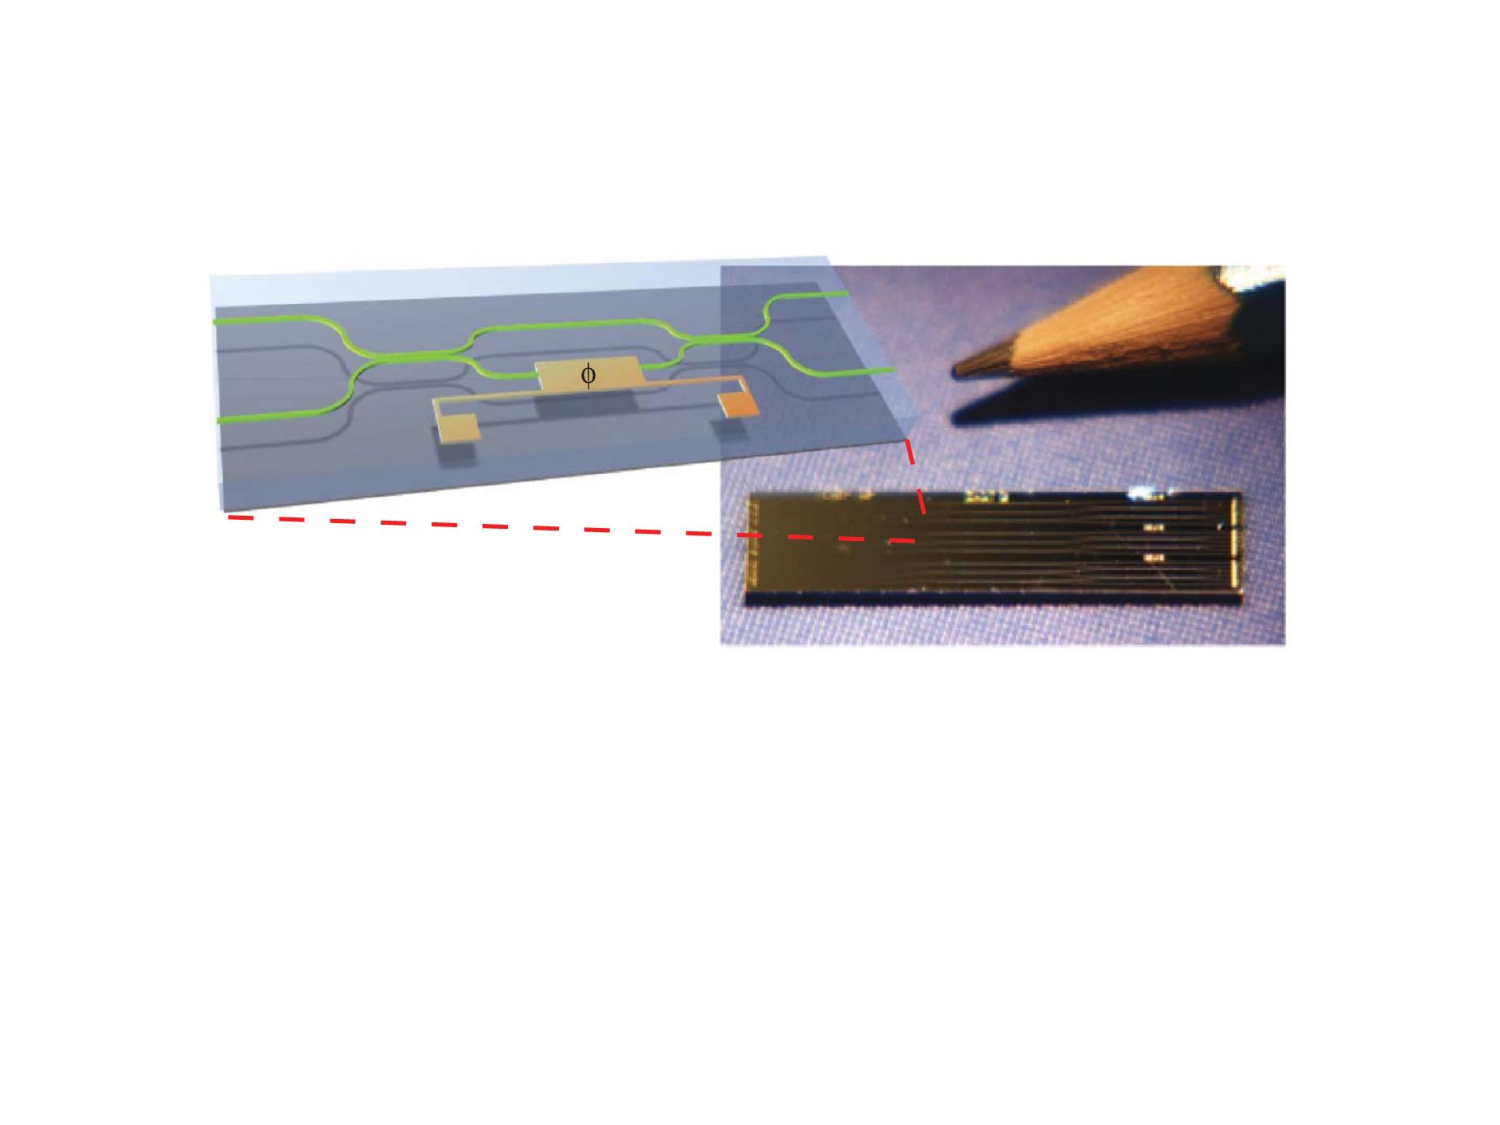
\includegraphics[width= 0.8\columnwidth]{figures/optics.pdf}
              \caption{光学量子计算机的示意图,一个微芯包含几块硅制波导干涉仪以及光控制相移器。绿色的线是光波导,黄色部分是金属制接触器。取自[Nature Photon. 3,
346 (2009)\cite{optics7}]
              }
              \label{photon}
            \end{center}
  \end{figure}

 \subsection{囚禁原子量子计算}

相对于其他体系,在囚禁原子和离子中,由于与环境的相互作用非常弱,所以该体系的退相干时间
非常长,典型的$T_2$已经为几秒,这是该体系作为量子计算方案的最大优势。

 在囚禁原子中,首先出现的是离子阱量子计算。把一个静电场和交变电场联合起来,然后将一串离子束缚于一个线性势阱之中。这些离子构成了qubit,而离子的两个能级则对应于qubit的两个态。单量子比特门
 可以通过对离子施加激光脉冲实现,而qubit之间的相互作用可以通过离子串的集体振动模式来传递,从而形成受控两比特门\cite{ions1,ions2}。2001年,Cirac和Zoller\cite{ions3}构想了利用
 许多独立离子阱以及一个用作探头的独立离子形成一个二维阵列,然后利用适当的激光脉冲可以将独立离子和选定的离子纠缠起来,从而实现可扩展的离子阱计算机。目前,实验上已经相继
 实现了八离子纠缠\cite{ions4}以及十四离子纠缠\cite{ions5}。

 中性原子的qubit和离子阱类似。首先激光束交叉构成一个光晶格,而中性原子就被囚禁在这些光晶格中\cite{atoms1}。qubit被编码在原子的能级上,可以通过光泵浦和激光冷却进行初始化,
 用电磁辐射进行操控,然后通过激光诱导荧光谱读出。但是目前为止,对光晶格中的中性原子的单独控制和测量在实验上还是非常困难的,
 但很多实验结果已经在这方面给出了相当广阔的前景\cite{atoms2,atoms3,atoms4,atoms5,atoms6}。
\begin{figure}[htbp]
            \begin{center}
              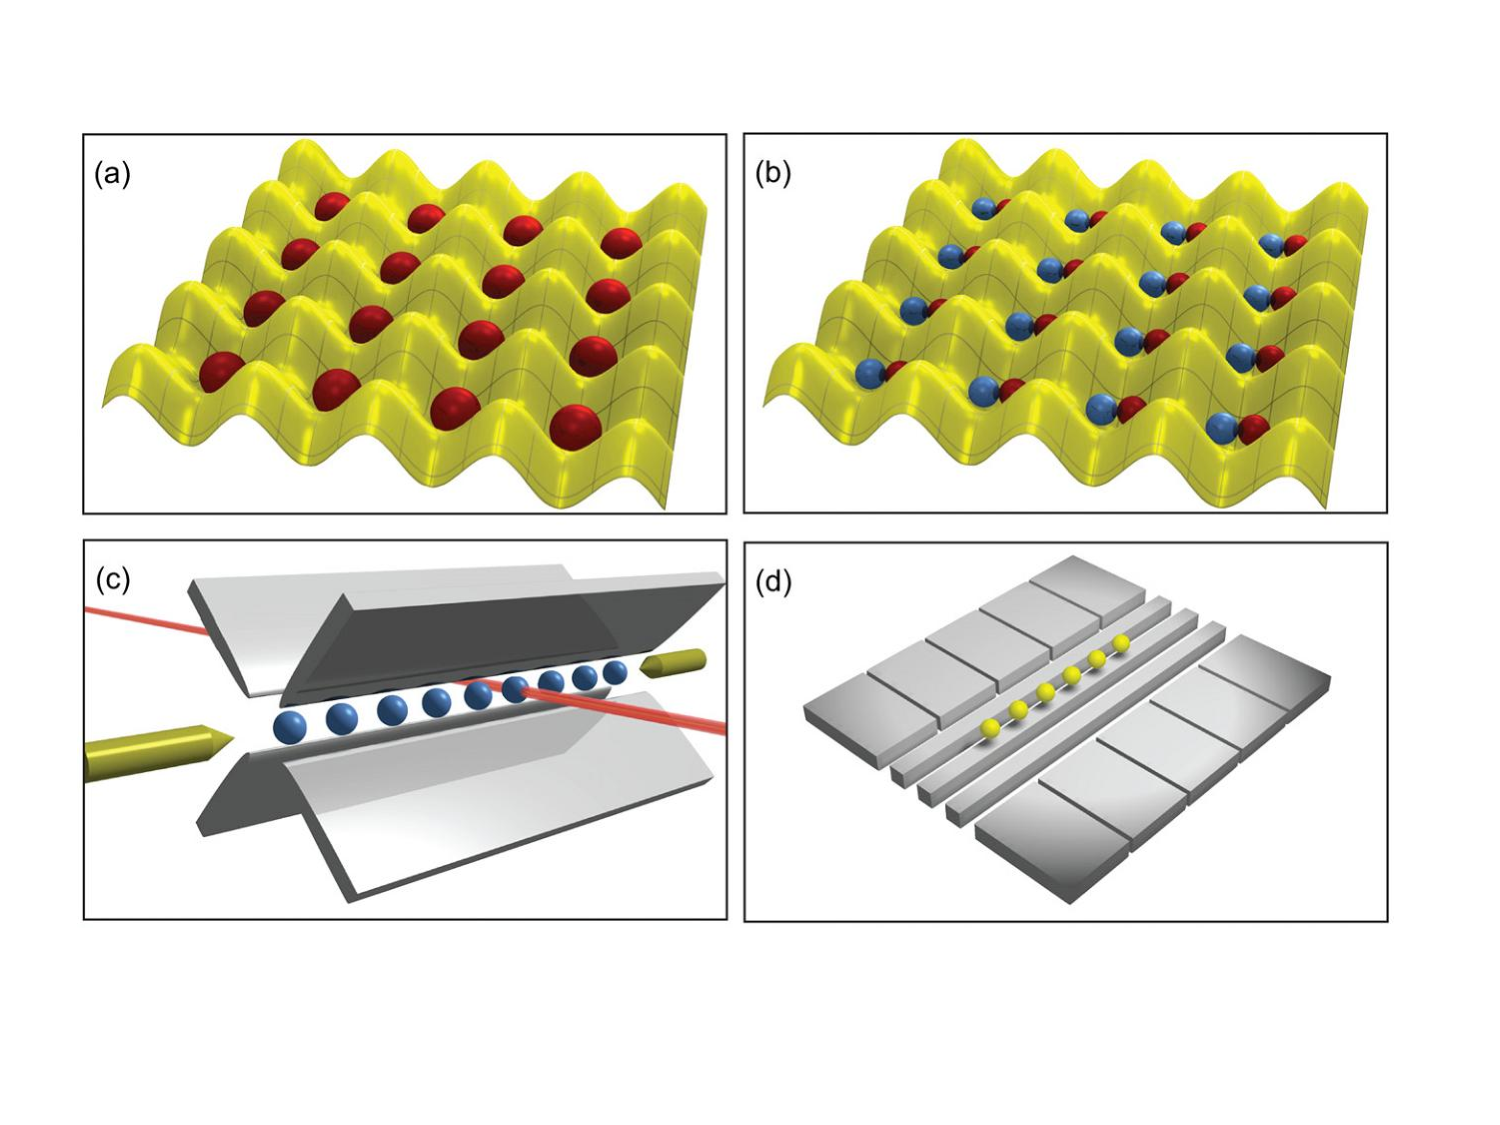
\includegraphics[width= 0.8\columnwidth]{figures/trap.pdf}
              \caption{(a)在周期光势阱中囚禁中性原子的方案。每一个中性原子是一个qubit,被囚禁在每个晶格中;(b)  可行的在中性原子中产生多粒子纠缠的方案,两个处于不同自旋态的原子束缚于同一个晶格中;(c) 线性势阱的示意图。处于同一个势阱中的离子拥有相同的振动模式,可以用来传递能量从而实现纠缠; (d) 平面势阱的示意图。近期发展的微米级离子阱技术对于在二维和三维上操控离子位置提供了相当大的便利。 取自[Rep. Prog. Phys. 74, 104401 (2011)\cite{review2}]
              }
              \label{trap}
            \end{center}
  \end{figure}

\subsection{超导线路量子计算}

超导线路典型的是$\mu$m尺度,并且是在mK温度下操作。虽然超导线路是肉眼可见的,但它依然
表现出很多可以用来作量子计算的量子行为\cite{super1,super2,super3,super4}。在超导线路中,qubit有很多种编码的方式:
在孤立的岛上超导电子的数目可以用作电压(charge) qubit;电流的方向可以用作磁通(flux) qubit;线路中的振荡态 可以用作相位(phase) qubit。这些qubit可以通过微波,电压,磁场,电流等进行高精度控制,从而实现量子计算任务。
目前超导线路中已经可以实现一些简单的量子算法\cite{super5}并产生三比特的纠缠态\cite{super6,super7,super8}。

 \begin{figure}[htbp]
            \begin{center}
              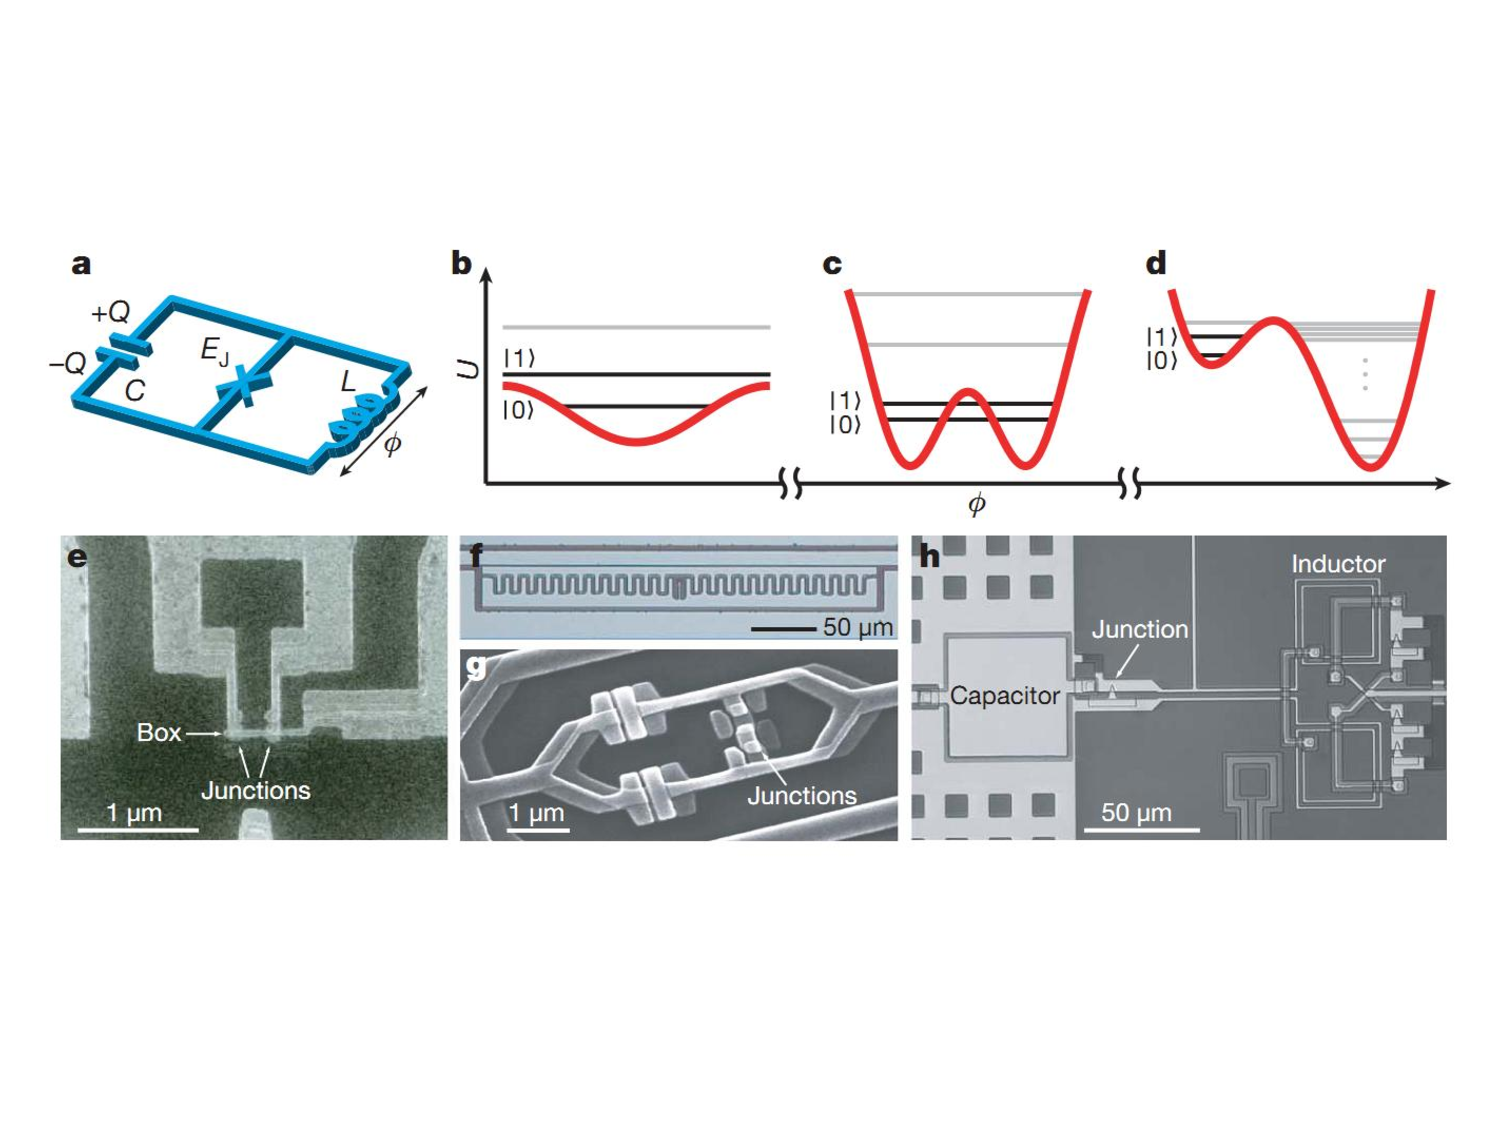
\includegraphics[width= 0.8\columnwidth]{figures/super.pdf}
              \caption{(a) 最小的超导线路模型,Josephson结用蓝色的“X”来表示;(b)-(d) Charge,flux和phase qubit中的势能(红色)以及能级(黑色);(e)-(h) 超导量子比特的微型照片。整个线路都是用铝薄膜制作的。e,f 为charge qubit,g为flux qubit,h为phase qubit。取自[Nature 464, 45 (2010)\cite{review1}]
              }
              \label{super}
            \end{center}
  \end{figure}

  \subsection{固态自旋量子计算}
当前的技术已经可以对固体中的单自旋进行相干操控和测量\cite{solid1,solid2},因此产生了
利用量子点中的电子自旋\cite{solid3}或者NV色心中的电子自旋及核自旋\cite{solid4}作量子计算的方案。
相比于其他体系,固态qubit的吸引力在于它们可以根据需要进行设计并且在大的阵列上进行扩展。
而且,固态方案要求的温度一般可以到几K的量级,NV色心更是可以在室温下进行操控。操控和读出的方法既可以
是电学手段\cite{solid5},也可以是光学手段\cite{solid6,solid7,solid8}。

虽然目前Rabi振荡已经可以在实验上被观测到\cite{solid9,solid10},但目前只有NV色心可以实现两比特门\cite{solid11},量子点中
只有一个逻辑态间的SWAP门在实验上实现了\cite{solid12}。NV色心中电子与核自旋之间纠缠起来也已在实验上实现\cite{solid13}。
\begin{figure}[htbp]
            \begin{center}
              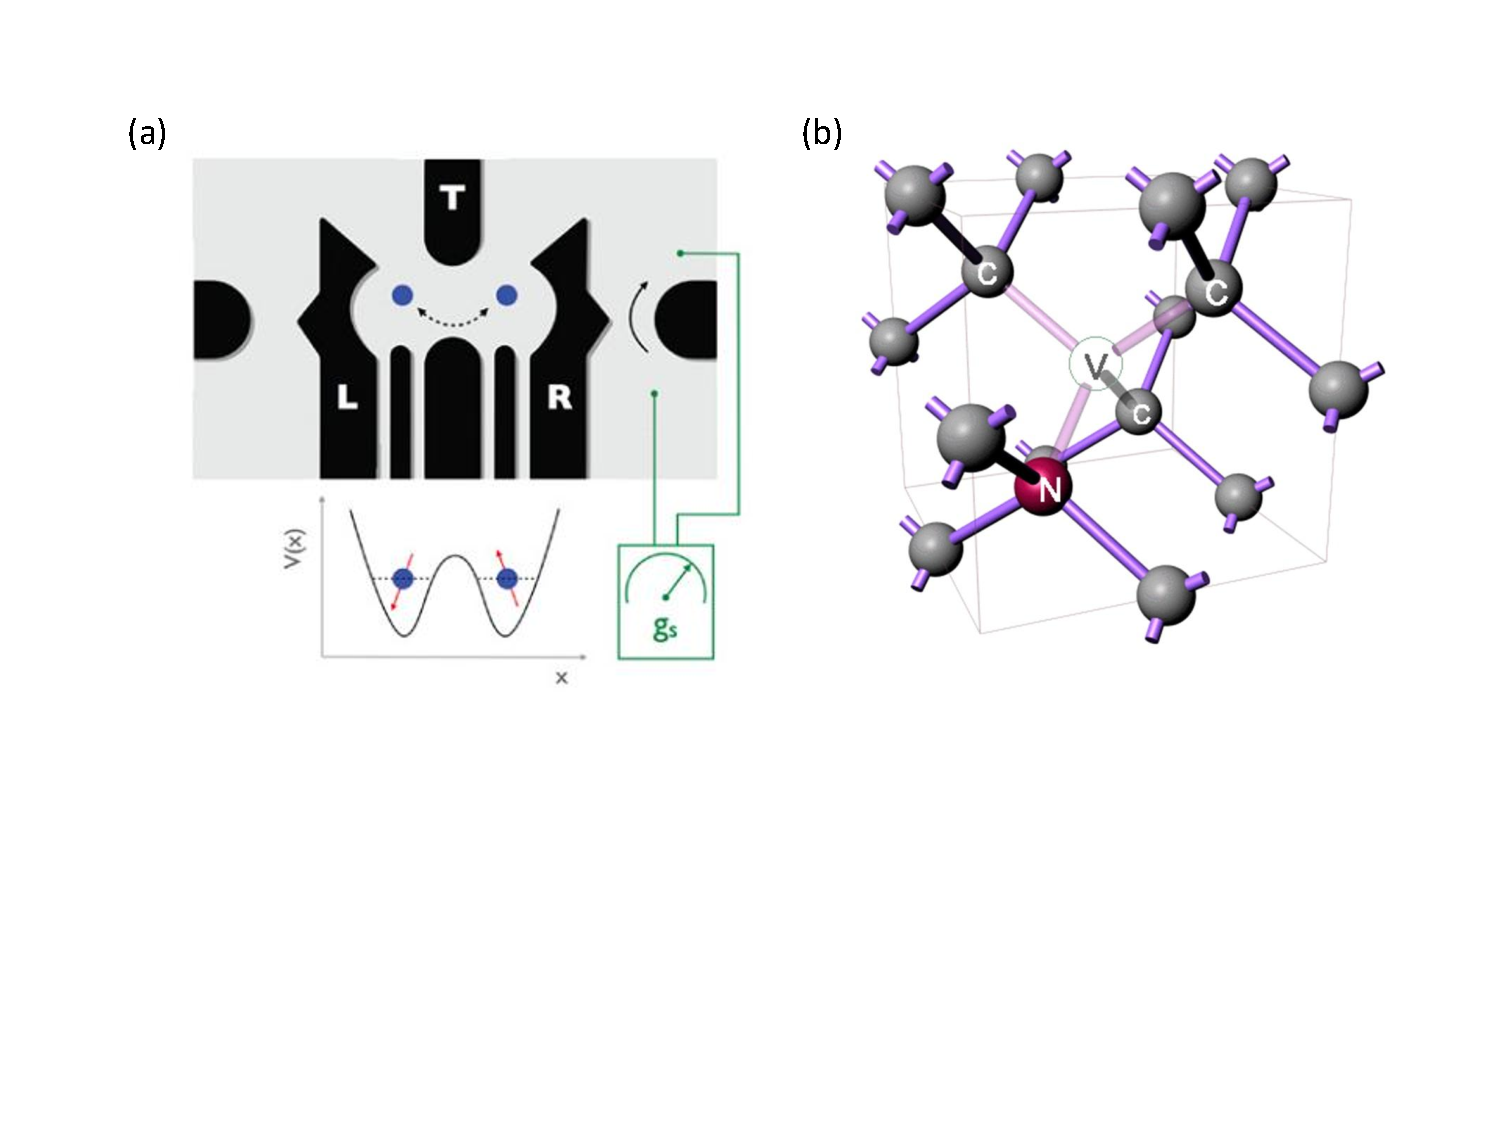
\includegraphics[width= 0.8\columnwidth]{figures/solid.pdf}
              \caption{(a) 两个电子的自旋态囚禁在半导体的双量子点结构上可以构成很好的qubit。传统的方法中,用磁场来操控qubit,但最近也发展了用电场操控的技术。取自[Rep. Prog. Phys. 74, 104401 (2011)\cite{review2}。
               (b) 金刚石中的NV色心,电子自旋可以通过磁场和可见光频率的电磁场来进行操控。取自[Phys. Rev. Lett. 93, 130501 (2004)\cite{solid11}]
              }
              \label{solid}
            \end{center}
  \end{figure}

\subsection{核磁共振量子计算}
液体溶剂中分子的核自旋非常适合做量子计算。分子的快速运动保证了该方案的$T_2$时间可以达到几秒的量级,媲美离子阱。1997年,第一次提出可以用已经存在发展了
超过50年的核磁共振技术做量子计算\cite{nmrpro1,nmrpro2}。在把样品置于核磁谱仪的强磁场中后,处于不同化学环境的核自旋可以通过Larmor进动频率分开。单比特门可以通过
外加射频脉冲实现,而两比特门可以通过核与核之间的相互作用来实现。目前,液体核磁已经可以实现最大到十二个qubit的量子计算\cite{12qubit},也已经验证了很多量子算法方案\cite{shor15}。
核磁共振遭遇的主要是可扩展性问题,想做到几十到上百个qubit理论上非常困难。
\begin{figure}[htbp]
            \begin{center}
              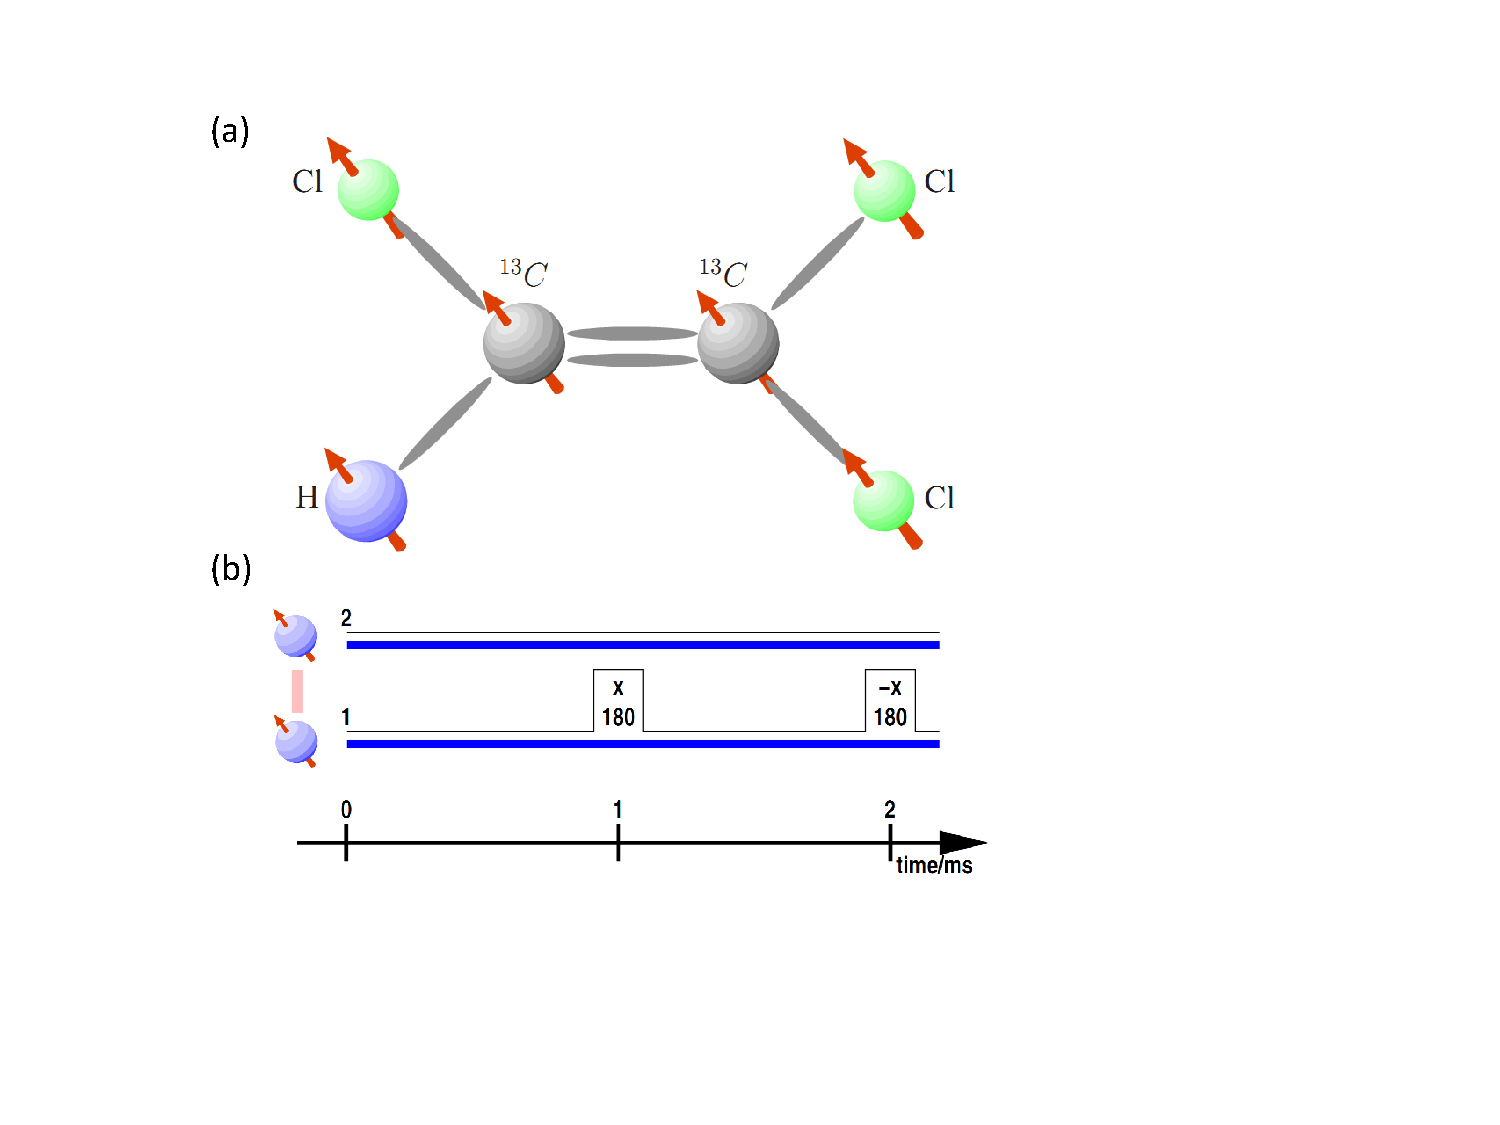
\includegraphics[width= 0.8\columnwidth]{figures/nmr.pdf}
              \caption{(a) 核磁共振中TCE分子的示意图。该分子中有三个可以用作自旋1/2的原子核,$^1$H和两个$^{13}$C。 (b)核磁共振中典型的脉冲序列示意图。该序列为耦合重聚的序列。取自[arXiv: 0207172 v1\cite{nmrreview1}]
              }
              \label{nmr}
            \end{center}
  \end{figure}

\subsection{各体系间的比较及展望}
展望未来,到底哪一个体系是最有希望实现真正的大尺度的量子计算机呢?这个问题非常难于回答,但我们首先要比较的就是各个体系的相干时间。我们给出了一个各体系之间的比较,总结于下图中。
\begin{figure}[htbp]
            \begin{center}
              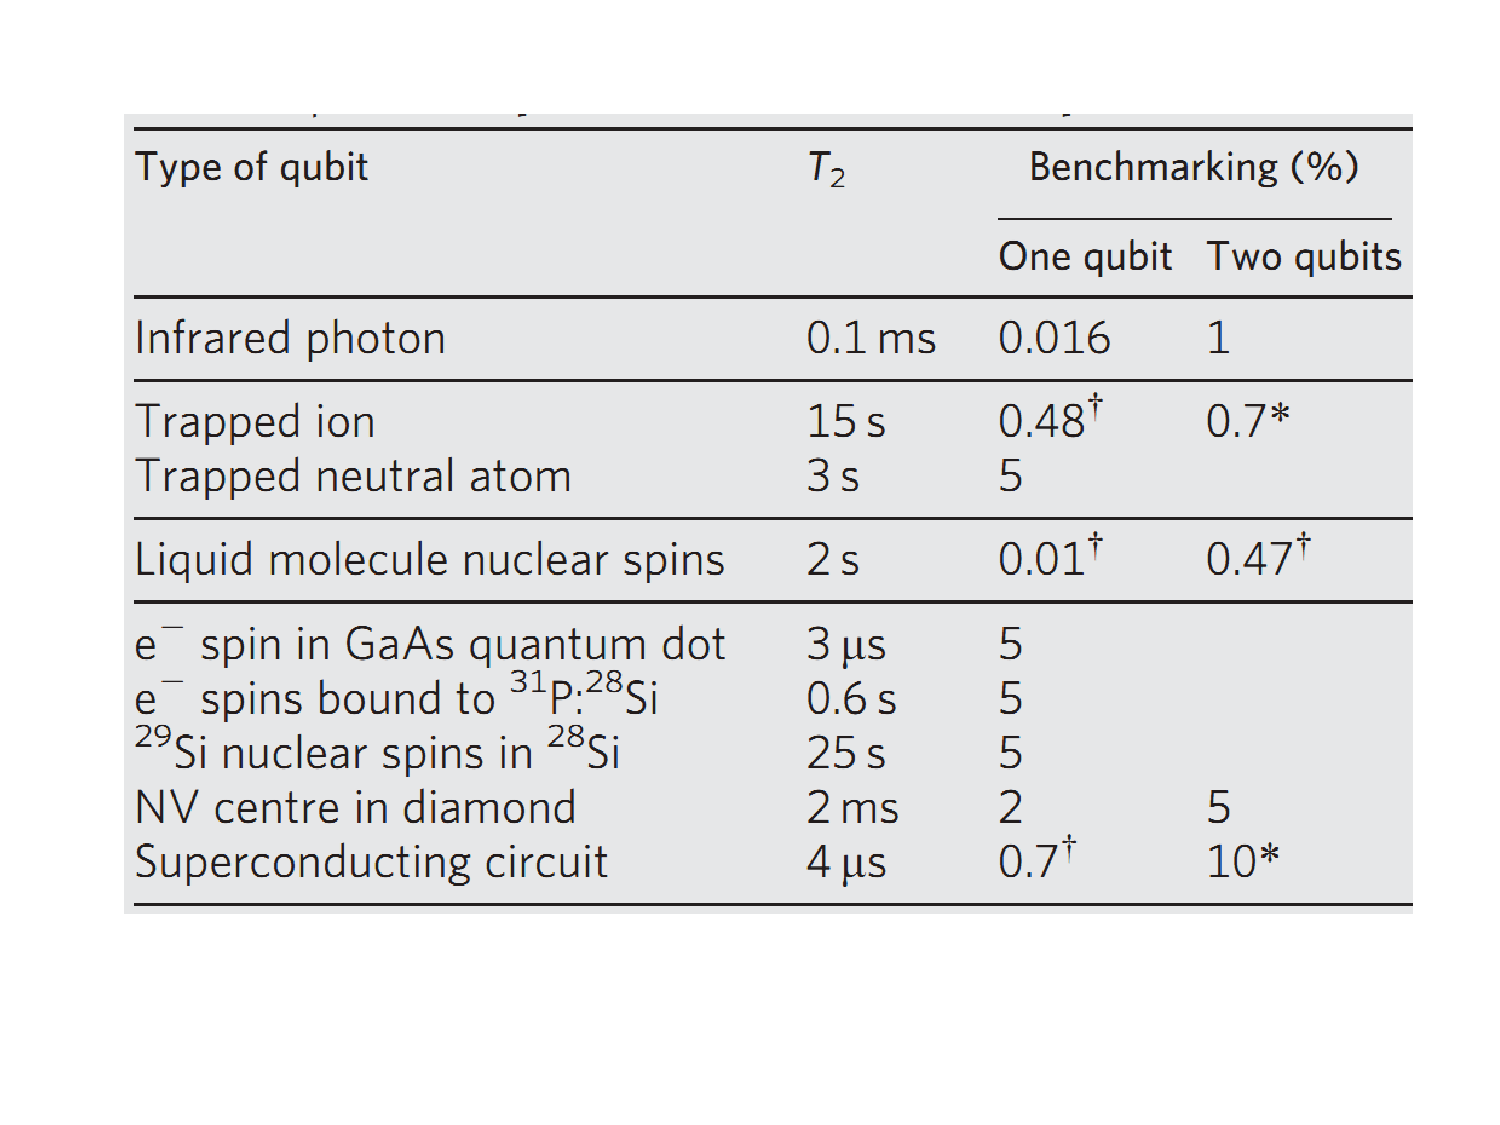
\includegraphics[width= 0.8\columnwidth]{figures/compare.pdf}
              \caption{各体系的$T_2$时间,以及逻辑门操作的保真度之间的比较。典型值给出的是单比特门和两比特门的错误概率,带$\ast$标记的数值是通过量子态重构或量子门重构得到的实验值,用100$\%$减去该值即为保真度。带$\dagger$标记的数值是通过随机基准
              (randomized benchmarking)过程获得。其他的数值则是粗略的对实验中操作误差的估计。取自[Nature 464, 45 (2010)\cite{review1}]。
              }
              \label{nmr}
            \end{center}
  \end{figure}
这些$T_2$时间可能随着技术的发展而增加,目前来看离子阱体系是最长的。当然,每个qubit的$T_2$还要和该体系的初始化,控制,以及测量时间相比较。

除了相干时间,在qubit的操控中的误差也是量子计算机必须考量的因素,这些数值也被总结在上表中。同时在逻辑门操作的时间内退相干的影响也是对逻辑门的误差有贡献的。还有各体系的量子纠错能力也是
要被考虑的因素,不过这个条件非常难以量化,它和机制复杂的噪声过程有关。

由于量子计算的实验进展是日新月异的,所以相关的参考文献最好选择最新的,比较推荐的有2010年Nature上的综述\cite{review1}以及2011年Rep. Prog. Phys.上的综述\cite{review2}。

\section{小结}

本章简略回顾了量子计算的发展历史,介绍量子计算机的工作原理以及当前实验上的进展。如果把经典计算机比喻为单一乐器的话,量子计算机就是一个交响乐团,你可以同时听到很多美妙的音乐;如果把经典计算机比喻为手动进水、漂洗、甩干的洗衣机的话,量子计算机就是
一台全自动洗衣机,只要“哔”的按下去脏衣服就一件一件变白了。但是,虽然量子计算机看上去很美好,但从目前的实验进展来看
建造一台真正的量子计算机的目标依然是很虚无缥缈的。这大概就和一个世纪前人们看待经典计算机的感觉一样。虽然很难,但我们一直在努力寻找新的方案,发展新的
技术,创造新的手段,等待所有的瓶颈都被突破的那一天。正如本章开始所说,创造一个会飞的马很难,但我们有一年的时间来努力,而一年确实是什么都有可能发生的,更何况我们用来
建造量子计算机的时间可不止一年,只要我们一直朝这个方向努力,总有一天我们会说,过去的电脑简直弱爆了,我们要玩量子并行版的Dota,我们要模拟自己的人生运势,当然闲来无事还要破解一下对门女孩子的QQ密码。

号称卖量子计算机的D-wave的广告词确实说的不错:

\emph{"Yes, you \textbf{can} have one."}

